\documentclass[thesis]{thesis-gwu}[2018/05/21]

\newcommand{\SO}[1]{\ensuremath{\mathrm{SO}(#1)}}
\newcommand{\SE}[1]{\ensuremath{\mathrm{SE}(#1)}}
\renewcommand{\so}[1]{\ensuremath{\mathfrak{so}(#1)}}
\newcommand{\Sph}{\ensuremath{\mathbb{S}}}
\newcommand{\norm}[1]{\ensuremath{\left\| #1 \right\|}}
\newcommand{\tr}[1]{\ensuremath{\mathrm{tr}\left( #1 \right)}}
\newcommand{\etr}[1]{\ensuremath{\mathrm{etr}\left( #1 \right)}}
\newcommand{\expect}[1]{\ensuremath{\mathrm{E}\left[ #1 \right]}}
\newcommand{\expectbar}[1]{\ensuremath{\bar{\mathrm{E}}\left[ #1 \right]}}
\newcommand{\cov}[2]{\ensuremath{\mathrm{cov}\left( #1, #2 \right)}}
\newcommand{\covbar}[2]{\ensuremath{\overline{\mathrm{cov}}\left( #1, #2 \right)}}
\newcommand{\expb}[1]{\ensuremath{\exp\left\{ #1 \right\}}}
\newcommand{\diff}{\ensuremath{\mathrm{d}}}
\newcommand{\diag}{\ensuremath{\mathrm{diag}}}

\newtheorem{definition}{Definition}[chapter]
\newtheorem{theorem}{Theorem}[chapter]
\newtheorem{lemma}{Lemma}[chapter]
\newtheorem{corollary}{Corollary}[chapter]

\DeclareMathAlphabet{\mathcal}{OMS}{cmsy}{m}{n}

\makeatletter
\newcommand\approxsim{\mathpalette\@approxsim\relax}
\newcommand\@approxsim[2]{%
	\mathrel{%
		\ooalign{%
			$\m@th#1\sim$\cr
			\hidewidth$\m@th#1:$\hidewidth\cr
		}%
	}%
}
\makeatother

% this package is only used to generate some random text. 
% it is not needed in a true document
\usepackage{lipsum}

% !TEX root = ../thesis-WW.tex

% --------- FRONT MATTER PAGES ---------------------
% Title of the thesis
\title{Geometric Formulation of Uncertainties and Estimation \\ for Three-Dimensional Rotations}

% Author name
\author{Weixin Wang}

% Previous degrees
\bsdepartment{Mechanical Engineering}
\bsschool{Tsinghua University}
\bsgrad{May 2016}

\msdepartment{Mechanical Engineering}
\msschool{University of Wisconsin-Madison}
\msgrad{December 2018}
\showmsdegree % you can show or hide the MS degree line 
% \hidemsdegree

% PhD degree commands
% Committee
\showcommitteepage % hide this page if you're doing a MS thesis
%\hidecommitteepage 
\committee{ %
Dr. Taeyoung Lee, Professor of Mechanical and Aerospace Engineering,\\ 
George Washington University, Dissertation Director\\ % remember to add a space between committee members

Dr. Kausik Sarkar, Professor of Mechanical and Aerospace Engineering, \\
George Washington University, Committee Chair\\

Dr. Peng Wei, Assistant Professor of Mechanical and Aerospace Engineering, \\
George Washington University, Committee Member\\

Dr. Chung Hyuk Park, Associate Professor of Biomedical Engineering, \\
George Washington University, Committee Member\\

Dr. Kyle DeMars, Associate Professor of Aerospace Engineering, \\
Texas A\&M University, Committee Member\\
}

% Chair must be entered separately for formatting reasons.
\chair{Taeyoung Lee}
\chairtitle{Professor of Mechanical and Aerospace Engineering}

% Uncomment the following lines if there are two dissertation co-directors.
%\hascochair
%\cochair{Murray Snyder}
%\cochairtitle{Professor of Mechanical and Aerospace Engineering}

% Department
\department{Mechanical and Aerospace Engineering}

\phdgrad{July 21, 2022}
\defensedate{July 21, 2022}
% Year of completion for copyright page and perhaps other places
\year=2022

% Copyright page
%\copyrightholder{Someone else}

% Dedication
%\dedication{ %
%Include a fancy quote or dedication
%}

% Acknowledgments
\acknowledgments{
    Here you can acknowledge all of those people who have helped you to reach this point.
    It's rare that any work is done in a vacuum and your research is no exception.
    Feel free to be grateful for all those who've aided you along your way.
}

% -----------------------------------------------------------------
% Typically only one of Preface/Foreward/Prologue would be in your thesis.
% To choose one simply delete the others and they will automatically dissappear

% ----------------------------------------------------------------------

% commands to show or hide front matter pages

\showcopyright
\showabstract
\showcommitteepage
%\showdedication
\showacknowledgments

% ------------ TABLE OF CONTENTS ----------------------
% Commands to hide or show lists of figures, tables, etc.
\showlistoffigures
\showlistoftables
\hidenomenclature

% --------- ACRONYMS and SYMBOLS ------------------------------
% TODO Deprecate the entire acronym package and switch to glossaries

% You can either use the acronymn or glossaries package (both work)
% Definition of any abbreviations used.
\abbreviations{
    \acro{CRTBP}{Circular Restricted Three Body Problem}
    \acro{NSA}{National Security Agency}
    \acro{SSME}{Space Shuttle Main Engine}
}
% call an abbreviation using \ac{abbrev}

% symbols and acronyms only show up when used in the text
\symbols{
    \acro{J}{Moment of Inertia}
}       

% if you want acronymn (simpler) then change these to show
\hidelistofabbreviations
\hidelistofsymbols

% if you want glossaries (more powerful) then leave above as hide
% GLOSSARIES package options - automatically turns off front pages from acronym package

% acronymns and symbols are basically the same, but there are two provided 
% locations where they can show up
\setabbreviationstyle[acronym]{long-short}
\setabbreviationstyle[abbreviation]{long-short}
\makeglossaries
% you can hide/show the glossaries page
\showglossarieslistofabbreviations
\showglossarieslistofsymbols
\showglossariesglossaryofterms

% acronyms defined in glossaries
\newabbreviation{crtbp}{CRTBP}{Circular Restricted Three Body Problem}
\newabbreviation{lidar}{LIDAR}{Light Detection and Ranging}
% defining abbreviations like this allows for autocompletion
\newglossaryentry{filo}{
    name={FILO},
    type=\glsxtrabbrvtype,
    description={first in last out},
    first={first in last out (FILO)}
}

% glossary entries
\newglossaryentry{linux}{
    name=Linux,
    description={is a generic term referring to the family of Unix-like computer operating systems that use the Linux kernel},
    plural=Linuces
}

\newglossaryentry{matrix}{
    name={matrix},
    plural={matrices},
    description={rectangular array of quanttities}
}

% symbols
\newglossaryentry{M}{
    type=symbols,
    name={\ensuremath{M}},
    sort=M,
    description={a \gls{matrix}}
}

\newglossaryentry{F}{
    type=symbols,
    name={\ensuremath{F}},
    sort=F,
    description={External Force}
}
% Some abstract text
\abstract{
This is the abstract. 
It contains some random text from the \texttt{lipsum} package. 
You may safely remove the \texttt{lipsum} package once you write your thesis.

\lipsum[1]
}


% this will speed up your tikz figures by building them once to another directory
\usepackage{pgfplots}
\usepgfplotslibrary{external}
\tikzexternalize
\tikzsetexternalprefix{cache/}

\usepackage{multirow}
\usepackage{siunitx}

%% DOCUMENT AREA
\begin{document}

% !TEX root = ../thesis-WW.tex

\chapter{Introduction} \label{chap:introduction}

\glsaddall

The 3D attitude of a rigid body is a key concept in modeling our physical world.
It can be defined as the directions of the three axes of an orthogonal frame fixed to the rigid body in the inertial frame, and therefore describes the orientation of the rigid body.
The attitude is a state involved with rigid body mechanics, and is usually controlled in a robotic system through actuators to achieve the goal of alignment or moving to a specific position.
As a feedback controller also needs the estimation of the state, a number of sensors are usually used to determine the attitude of the rigid body.
These sensors can usually be classified into the following categories:
(i) infrastructures that measure the attitude directly, for example an optical motion capture system;
(ii) a gyroscope that measures the angular velocity;
(iii) direction sensors that measure reference directions in the inertial frame, such as magnetometers, star trackers, etc;
(iv) sensors that measure the surrounding environment, such as various cameras, lidars, etc.

These sensors provide either direct or indirect information of the attitude of a rigid body.
But one common feature is that they are all subject to measurement noises.
The noise characteristics of different types of measurement are also different.
For example, the attitude integrated from angular velocity measured by a gyroscope suffers from accumulated integration of bias, and therefore it is reliable within a short period of time.
It is similar for a visual odometry algorithm that estimates the attitude by capturing surrounding visual features using cameras.
On the other hand, the attitude inferred from measurements of reference directions may be affected by instantaneous disturbances, but the average noise remains low for a long period of time.
Thus, it is common that different sensors are combined to obtain a robust attitude estimate, by leveraging their different noise characteristics.

This motivates the need to model the uncertainty of the attitude.
As when combining the estimates from two or more different measurement sources, one must decide how much confidence should be placed on each individual source.
As a rule of thumb, the measurement with more uncertainty should play a less important role in determining the final estimation.
Consequently, a metric that describes the uncertainty for the estimated attitude is needed to weigh the measurements.
From another point of view, uncertainty of the final estimation can play an important role in decision making for a robotic system.
For example, if the uncertainty for attitude is too large, a robot may take some safety measures like slowing down, to avoid possible collisions.

This dissertation focuses on modeling the uncertainty of the rigid body attitude in a geometric and global fashion.
More specifically, the uncertainty is formulated on the curved and compact manifold where the attitude naturally resides in an intrinsic fashion.
Furthermore, a model for the correlation between attitude and other Euclidean quantities, for example the 3D location, is proposed.
Based on these, three typical estimation problems in aerospace and robotics engineering are investigated: (i) attitude estimation with a gyroscope and direction sensors, (ii) loosely coupled IMU-GNSS integration for navigation, and (iii) visual-inertial navigation and odometry with an RGB-D camera. 

\section{Motivation and Goal}

In the existing algorithms for attitude estimation from different sensors, the uncertainty of attitude is usually modeled in two different ways.
In the first way, attitude parameterizations, such as Euler angles or quaternions, are treated directly as quantities in the Euclidean space, and the Gaussian distribution is used to model their uncertainty.
This method entirely ignores the geometric constraints on the attitude parameterizations, such as the singularity of Euler angles, or that a quaternion representing attitude should have unit norm.
As a result, its accuracy is typically low, and may have numerical issues associated with singularities, or that the covariance matrix becomes singular.

Instead of directly treating the attitude parameterizations as in Euclidean space, the more popular second approach treats the 3-dimensional parameterizations of attitude \textit{error} as in Euclidean space.
In this approach, since the attitude error is typically small, it avoids the singularity of the parameterization, which is usually at 180 degrees.
Also, by using the minimal three dimensional parameterization, it avoids an equality constraint that makes the covariance matrix for a unit quaternion singular.
The parameterizations frequently used include rotation vectors and modified Rodrigues parameters.

Although the second approach of modeling attitude uncertainty seems very reasonable, and usually achieves good estimation accuracy of attitude in practical applications, it still does not faithfully respect the geometric structure of the attitude space.
For example, the space of rotation vectors is actually cyclic, i.e., any rotation vectors with the same direction that differ in length by $2k\pi$, $k\in\mathbb{Z}$, represent the same rotation.
As a consequence, a Gaussian distribution for rotation vectors needs to be \textit{wrapped}, or \textit{folded} in order to faithfully represent the uncertainty.
Namely, the densities representing the same rotation need to be added up.
An example of a wrapped Gaussian distribution in the one dimensional rotation space is shown in Fig. \ref{fig:wrapping}.
If the uncertainty is low, or the variance of the Gaussian distribution is small, the error caused by wrapping can usually be neglected.
However, for large uncertainty, as indicated in Fig. \ref{fig:wrapping}, wrapping makes the uncertainty much larger than that indicated by the original Gaussian distribution.

\begin{figure}
	\centering
	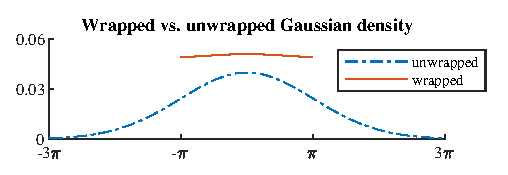
\includegraphics[scale=1.2]{figures/wrapping}
	\caption[Gaussian density vs. wrapped Gaussian density.]{Gaussian density vs. wrapped Gaussian density with $\mu=0$ and $\sigma^2=10$.
		The wrapped Gaussian distribution is defined in the circular space $\mathbb{R}/2\pi$ by identifying $\theta$ with $\theta+2k\pi$ for $k\in\mathbb{Z}$, so the densities beyond $[-\pi,\pi]$ are wrapped into $[-\pi,\pi]$. \label{fig:wrapping}}
\end{figure}

In this dissertation, an alternative approach is sought to model large uncertainty of rigid body attitude, which cannot be accurately described by a Gaussian distribution as discussed above.
The key idea is that instead of treating parameterizations of attitude as quantities in Euclidean space, a probability density defined directly in the space of attitude is used.
Classic densities include the matrix Fisher distribution defined on the three dimensional special orthogonal group $\SO{3}$, and the Bingham distribution defined on the unit three sphere $\Sph^3$.
In this way, the geometric constraints on the parameterizations of attitude are completely avoided, and the densities are suitable for arbitrarily large uncertainty including a uniform distribution, which is made possible by the compactness of the attitude space.

To apply these densities in estimation problems encountered in engineering, the correlation between attitude and other Euclidean quantities must also be considered, since attitude is usually jointly estimated with these quantities, such as the gyroscope bias, and the position.
This issue is investigated in this dissertation by introducing a new probability density defined on $\SO{3} \times \mathbb{R}^n$, referred to as the matrix Fisher--Gaussian (MFG) distribution.
With this new tool, classic estimation problems in engineering, including attitude determination and localization, can be tackled with probabilistic models that fully respect the underlying geometric structure of the attitude space.
Therefore, in the presence of large uncertainty, for example unknown initial conditions, estimators can converge with a much faster speed than the conventional Gaussian approach, thanks to the accurate modeling of large uncertainty.

\section{Literature Review}

Probabilistic models that describe uncertainty on curved manifolds have been studied by statisticians in the branch called \textit{directional statistics}.
In this section, the developments in directional statistics that are relevant to this dissertation are reviewed.
Then, classic methods for rigid body estimation using gyroscopes and direction sensors are introduced.
Moreover, some attempts in applying the matrix Fisher distribution, and Bingham distribution to attitude estimation are examined.
Finally, the progresses in rigid body pose estimation (attitude and position) using various cameras with an IMU (inertial measurement unit), are reviewed.

\subsection{Directional Statistics} \label{section:intro-review-direction}

Although the Gaussian distribution is the dominate probabilistic model in both theoretical research and practical engineering, it falls short when the data of interest are on a curved manifold, such as the unit sphere $\Sph^2$, and the special orthogonal group $\SO{3}$.
Statisticians have proposed new models directly defined on these manifolds, to replace the Gaussian distribution when the uncertainty of data is large.
The materials in this subsection are mostly based on the book \cite{mardia2009directional}.
Another useful exposition of models on the Stiefel and Grassmann manifolds can be found in \cite{chikuse2003statistics}.

\paragraph{Models on Unit Circle and Sphere}

One of the most frequently encountered and simplest manifold is the one dimensional unit circle: $\Sph^1 = \{ x\in\mathbb{R}^2 \,|\, \norm{x} = 1 \}$.
Any element on the unit circle can be written as an angle $\theta\in\mathbb{R}$, however, $\theta$ and $\theta+2k\pi, k\in\mathbb{Z}$ represent the same element due to the cyclic nature of $\Sph^1$.
As a consequence, the unit circle can also be regarded as the space of one dimensional rotation, i.e., the two dimensional special orthogonal group $\SO{2} = \{ R\in\mathbb{R}^{2\times 2} \,|\, RR^T = I_{2\times 2},\, \det R = 1\}$, where
\begin{align*}
	R = \begin{bmatrix}
		\cos\theta & -\sin\theta \\
		\sin\theta & \cos\theta
	\end{bmatrix}.
\end{align*}
Various probability densities have been developed on $\Sph^1$, such as the von Mises distribution \cite{von1918uber}, wrapped normal (Gaussian) distribution, wrapped Cauchy distribution, projected normal distribution (angular Gaussian distribution), etc.
The first three distributions are uni-modal and have similar shapes (see \cite[Figure 3.3]{mardia2009directional}), whereas the last can be bi-modal.
Among these, the von Mises distribution is one of the most frequently used models, and can be regarded as an analogue of Gaussian distribution on $\Sph^1$, due to their several similarities.

The von Mises distribution can be generalized into (hyper) unit spheres $\Sph^n = \{ x\in\mathbb{R}^{n+1} \,|\, \norm{x}=1 \}$, for $n\geq 2$, and is usually named as von Mises--Fisher distribution \cite{fisher1953dispersion}.
If $x\in\Sph^n$ follows a von Mises--Fisher distribution, it has the following density function
\begin{align*}
	p(x) = \left(\frac{\kappa}{2}\right)^{(n+1)/2-1} \frac{1}{\Gamma((n+1)/2) I_{(n+1)/2-1}(\kappa)} \expb{\kappa\mu^T x}
\end{align*}
with respect to the uniform distribution, where $\mu\in\Sph^n$, $\kappa>0$ are the parameters of the distribution, $\Gamma$ is the gamma function, and $I_\nu$ is the modified Bessel function of the first kind with order $\nu$.
For the unit sphere $\Sph^2$, the density function reduces to
\begin{align}
	p(x) = \frac{\kappa}{\sinh\kappa} \expb{\kappa\mu^T x}.
\end{align}
This distribution is denoted by $x\sim \mathcal{VM}(\mu,\kappa)$.
The parameter $\mu$ represents the mean direction, and $\kappa$ represents the concentration, with larger $\kappa$ meaning higher concentration.
The von Mises--Fisher distribution is used to model the uncertainty of direction measurements in this dissertation.

\paragraph{Models on $\SO{3}$}

Another frequently encountered manifold in engineering and material science is the space of 3D rotations, i.e., the three dimensional special orthogonal group: $\SO{3} = \{ R\in\mathbb{R}^{3\times 3} \,|\, RR^T = I_{3\times 3}, \, \det R = 1\}$.
One of the most famous models on $\SO{3}$ is the matrix Fisher distribution \cite{downs1972orientation,khatri1977mises}, which is originally defined on the Stiefel manifolds, i.e., an orthogonal $r$ frame in $\mathbb{R}^n$ with $r\leq n$.
When $r=2$, $n=3$, the Stiefel manifold is $\SO{3}$ \cite[Chapter 13.2.1]{mardia2009directional}.
Similar to von Mises distribution, the matrix Fisher distribution can be regarded as an analogue of the Gaussian distribution on $\SO{3}$.

Any 3D rotation can also be parameterized by a unit quaternion $q\in\Sph^3$.
The space of unit quaternions $\Sph^3$ forms a double cover of $\SO{3}$, therefore, $q$ and $-q$ represent the same 3D rotation.
The Bingham distribution \cite{bingham1974antipodally} is formulated on $\Sph^n$, $n\geq 1$ with antipodal symmetry, i.e., the densities for $x$ and $-x$ are identical.
Thus, the Bingham distribution on $\Sph^3$ can be treated as a probability distribution on $\SO{3}$.
In fact, it has been shown to be equivalent to the matrix Fisher distribution on $\SO{3}$ \cite{prentice1986orientation}.
The definition, construction, and properties of these two distributions will be introduced in detail in Chapter \ref{chap:MF}.

Besides these two popular models, a ``normal'' like distribution on $\SO{3}$ is proposed in \cite{nikolayev1997normal} using the central limit theorem,
the Cayley distribution is introduced in \cite{leon2006statistical} using the Cayley transform,
and some other density functions are formulated in \cite{bunge2013texture,matthies1982form}.
These (including the matrix Fisher distribution) are further summarized under a generic approach of constructing probability distributions on $\SO{3}$ proposed in \cite{qiu2014wrapped} based on the exponential map, called the UARS model.
Moreover, the authors in \cite{qiu2014wrapped} introduced the wrapped tri-variate normal distribution on $\SO{3}$, generalizing the wrapped normal distribution on $\Sph^1$ by assuming the rotation vector follows a Gaussian distribution.

\paragraph{Correlations with Euclidean Space}

In practical applications, data on manifolds are usually coupled with other data in the Euclidean space, such as the attitude and position of a rigid body.
Therefore, it is also necessary to model the correlation between the manifold and Euclidean space.
In \cite{mardia1978model}, the von Mises distribution on $\Sph^1$ and the Gaussian distribution on $\mathbb{R}^1$ are coupled to define a density on the cylinder $\Sph^1 \times \mathbb{R}^1$, where some other models \cite{abe2017tractable,johnson1978some,kato2008dependent} have also been introduced to model the correlation between $\Sph^1$ and $\mathbb{R}^1$.
In addition, the von Mises distribution has also been generalized to multi-variate von Mises distribution \cite{mardia2008multivariate} to model the correlation between pairs of several random angles in $\Sph^1$.

There have also been two attempts to couple $\SO{3}$ and $\mathbb{R}^n$.
In \cite{markley2006attitude}, the matrix Fisher distribution is coupled with the Gaussian distribution by making the parameter of the matrix Fisher part dependent on the random variable in the Euclidean space.
The same approach has also been used to couple the Bingham distribution and Gaussian distribution \cite{darling2016uncertainty}.
However, this coupling technique, although being reasonable, is not originated from a generic geometric construction principle.
As a consequence, these models require very difficult computations when applied to practical problems, especially numerical optimizations are required when performing maximum likelihood estimation, i.e., recovering parameters from data, which limits their applications.

\subsection{State Estimation on $\SO{3}$} \label{section:intro-review-estimation}

Rigid body attitude estimation is the basic algorithm for numerous robotics and aerospace applications, and has been studied extensively by researchers and practitioners.
For example, in inertial navigation, the acceleration measurement must be first transformed into the inertial frame, which requires the attitude of the accelerometer to be estimated.
For a bipedal robot, its inclination must be first estimated so that the controller can prevent it from falling.
For a telescope operating in space, such as the Hubble telescope, its attitude must be known to direct its lens to a specific area of space.

Attitude estimation algorithms can be divided into the following three categories:
(i) deterministic observers with guaranteed convergence;
(ii) nonlinear Kalman filter based stochastic filters;
and (iii) stochastic filters based on the matrix Fisher and Bingham distributions.
But before reviewing these three categories, attitude parameterizations must be first introduced.

\paragraph{Attitude Parameterizations}

The attitude of a rigid body has three degrees of freedom.
However, a rotation matrix $R\in\SO{3}$ has 9 parameters, and is therefore subject to 6 equality constraints.
Due to its redundancy, few stochastic filters directly operate on rotation matrices.
Instead, people seek for attitude representations with fewer parameters.
A comprehensive review on this topic is given in \cite{shuster1993survey}.
Nevertheless, it should be noted that it is topologically impossible to have a global 3-dimensional parameterization without singular points for $\SO{3}$ \cite{stuelpnagel1964parametrization}.
Moreover, 5 is the minimum dimension of parameterizations to represent $\SO{3}$ in a one-to-one and global fashion \cite{stuelpnagel1964parametrization}.

Perhaps the most popular 3-dimensional parameterization of attitude is Euler angles.
The Euler angles have 24 different forms depending on the sequence of rotations, and in which frame the rotations are formulated (intrinsic and extrinsic).
The intrinsic z-y-x Euler angles are usually used in aerospace engineering, which are also referred to as the yaw, pitch, and roll angles.
The singular point for this set of Euler angles is when the pitch angle is 90 degrees, which is famously known as the gimbal lock.

Another frequently used 3-dimensional parameterization is the rotation vector.
By the Euler's rotation theorem, any 3D rotation can be described by rotating about an axis $u\in\Sph^2$ by an angle $\theta\in\mathbb{R}$.
And the rotation vector is simply $v = \theta u \in \mathbb{R}^3$.
The singular point for rotation vectors is when $\norm{v} = \theta = \pi$, i.e., when the rotation angle is 180 degrees.
Two other 3-dimensional parameterizations that are used in aerospace engineering are Rodrigues parameters and modified Rodrigues parameters, given by $\rho = \tan(\theta/2) u \in \mathbb{R}^3$, and $p = \tan(\theta/4) u \in \mathbb{R}^n$, respectively.
The singular points for these two parameterizations are when $\theta = \pi$, and $\theta = 2\pi$, respectively.

As mentioned in Section \ref{section:intro-review-direction}, the attitude can also be parameterized using unit quaternions in $\Sph^3$.
This is a 4-dimensional singularity free parameterization, and is widely used in attitude estimation algorithms.
The unit quaternion corresponding to the rotation $(u,\theta)$ can be written as
\begin{align} \label{eqn:rv2qua}
	q = \begin{bmatrix} \cos(\theta/2) \\ \sin(\theta/2) u \end{bmatrix} \in \Sph^3
\end{align}
in the Hamilton convention.
It should be noted that $q$ and $-q$ represent the same 3D rotation.

\paragraph{Deterministic Observers}

This type of attitude estimators assume all measurements are noise free, so the convergence from a wrong initial attitude to the true attitude can be proved using a rigorous Lyapunov argument.
Typically, it is assumed that the angular velocity is measured by a gyroscope, so that the attitude can be integrated forward in time.
Also, various reference directions in the inertial frame are measured in the reference frame fixed to the rigid body (body-fixed frame), to correct the initial and integration errors.

The first and most famous attitude observer with guaranteed convergence is proposed in \cite{mahony2008nonlinear}.
This observer has been extensively used in attitude controllers for unmanned aerial vehicles.
Later, it has been generalized to deal with reference directions that are time varying in the inertial frame \cite{batista2012ges,grip2011attitude,trumpf2012analysis}.
Also, a hybrid correction scheme has been proposed in \cite{wu2015globally} to deal with the zero measure set where the initial attitude does not converge for the observer in \cite{mahony2008nonlinear}.
Moreover, the rotation of the Earth has also been incorporated to enhance attitude observability when only a single reference direction is available \cite{reis2018nonlinear}.

\paragraph{Nonlinear Kalman Filters}

Different from deterministic observers, stochastic filters assume that both the gyroscope and direction measurements are subject to noises.
And the filter determines how many weights are given to the integrated attitude and the direction measurements, based on their respective covariance matrices.
Compared to deterministic observers, filters typically have faster convergence rate when the initial uncertainty, and sensor noise characteristics are known.
On the other hand, due to the difficulty of formulating stability under stochastic settings \cite{karvonen2020stability}, convergence properties are usually not studied for stochastic filters.

A comprehensive review of attitude estimation algorithms based on extended Kalman filters (EKF) and unscented Kalman filters (UKF) has been presented in \cite{crassidis2007survey}.
The EKF can be naturally applied to attitude kinematics formulated in Euler angles \cite{farrell1970attitude,foxlin1996inertial}, Rodrigues parameters \cite{idan1996estimation}, and modified Rodrigues parameters \cite{crassidis1996attitude}.
However, due to the singularity of 3-dimensional attitude parameterizations, these filters must be operated in a limited range of attitude, which cannot undergo continuous spinning.
Also, a less noticed problem is that the Lebesgue measure in $\mathbb{R}^3$ for these parameterizations does not correspond to a uniform measure on $\SO{3}$, which means that the Gaussian distribution in $\mathbb{R}^3$ is no longer Gaussian shaped on $\SO{3}$, and this causes inaccuracy in modeling the uncertainty.

The problem caused by singularity is avoided by the celebrated multiplicative EKF (MEKF) \cite{lefferts1982kalman,markley2003attitude}.
Instead of directly working with 3-dimensional attitude parameterizations, MEKF treats a 3-dimensional parameterization of \textit{attitude error} as the state vector.
More specifically, a unit quaternion $q$ is used as the estimated attitude, and an attitude error parameterized by one of the 3-dimensional parameterizations (rotation vectors, Rodrigues and modified Rodrigues parameters) is used to model the uncertainty of the estimated $q$.
The term ``multiplicative'' refers to the multiplication between the estimated quaternion and the attitude error:
\begin{align} \label{eqn:attitude error representation}
	q_t = q \otimes \delta q\{v\},
\end{align}
where $q_t$ is the true quaternion, $\delta q\{v\}$ is the error quaternion corresponding to the 3-dimensional parameterization $v\in\mathbb{R}^3$, and $\otimes$ is the quaternion multiplication.
Because the attitude error $v$ is usually small, it avoids the singularity of the parameterization.

MEKF remains one of the most robust and efficient attitude filters, which has been validated by several NASA space missions \cite{crassidis2007survey}.
The unit quaternion $q$ in MEKF can be replaced by a rotation matrix $R$ without changing the structure of the filter.
Also, in \eqref{eqn:attitude error representation}, the attitude error $v$ is expressed in the body-fixed frame, and it can be changed into the inertial frame by reversing the order of multiplication
\begin{align} \label{eqn:attitude error representation-inertial}
	q_t = \delta q\{v\} \otimes q.
\end{align}
This convention has some advantages over \eqref{eqn:attitude error representation} \cite{gai1985star,li2012improving} which potentially injects some false information from the measurement when there is an unobserved degree of freedom.
A second order MEKF has also been studied in \cite{markley2003attitude}, and an unscented Kalman filter parallel to MEKF has been proposed in \cite{crassidis2003unscented}.

In contrast to MEKF, the quaternion can also be directly treated as the state vector of an EKF, so that the attitude error becomes addictive
\begin{align}
	q_t = q + \delta q,
\end{align}
which is referred to as the addictive EKF (AEKF).
The comparison of MEKF and AEKF has been studied in \cite{markley2004attitude,shuster2003constraint2,shuster2003constraint1}.
However, normalizing the quaternion to have unit norm by brute force in AEKF makes the covariance matrix for quaternions singular, and should be avoided.
On the contrary, identifying quaternions on the same line through the origin in $\mathbb{R}^4$ without the unit norm constraint makes AEKF equivalent to MEKF, although it is not suggested due to the increased computation \cite{markley2004attitude}.

The idea of MEKF has been generalized to the estimation problem of both attitude and position of a rigid body \cite{sola2017quaternion}, which establishes a framework for Kalman filter based inertial navigation.
Also, using the ``error state'' to represent uncertainty has been more formally studied on matrix Lie groups as the invariant extended Kalman filter (IEKF) in \cite{barrau2014intrinsic,barrau2016invariant,barrau2018invariant}.
In particular, it is proved in \cite{barrau2016invariant} that IEKF is stable when acting as an observer on matrix Lie groups, similar to a linear Kalman filter.

\paragraph{Filters Based on Directional Statistics}

Although MEKF achieves great success in attitude estimation, it cannot deal with large uncertainty due to the underlying Gaussian assumption of the 3-dimensional parameterization of attitude error, discussed at Figure \ref{fig:wrapping}.
This disadvantage can be overcome by replacing the Gaussian distribution using the probability distributions defined directly on $\SO{3}$ from directional statistics, namely the matrix Fisher and Bingham distributions.

The attitude filter based on the Bingham distribution was proposed independently in \cite{glover2014tracking} and \cite{kurz2014recursive}.
Later, the attitude filter based on the matrix Fisher distribution was proposed in \cite{lee2018bayesian}.
Given that the two distributions are equivalent, these filters are also equivalent, except some differences in numerical implementations.
Furthermore, attitude filters using deterministic sampling of sigma points were developed in \cite{gilitschenski2015unscented} and \cite{lee2018bayesian} for the two distributions respectively, similar to UKF.
The Bingham distribution has also been generalized into dual quaternions to represent the uncertainty of attitude and position simultaneously in \cite{arun2018probabilistic,gilitschenski2014new,li2019geometry,li2020unscented}.
This approach deals with the correlation between attitude in $\SO{3}$ and position in $\mathbb{R}^3$.
However, the correlation must respect the structure of three dimensional Euclidean group $\SE{3}$ when it is used, hence it cannot deal with Euclidean random variables other than position.

In \cite{markley2006attitude}, an attitude filter was proposed using a new probability density on $\SO{3}\times \mathbb{R}^n$ where the attitude part is a matrix Fisher distribution, so that all sensor biases can be estimated concurrently with attitude.
However, the quadratic terms appeared in the uncertainty propagation and measurement update steps must be omitted to make the density function closed under the proposed functional form, which lacks theoretical soundness.
In addition, an uncertainty propagation scheme based on the proposed Gauss-Bingham distribution was introduced in \cite{darling2016uncertainty}, which can also deal with the correlation between $\SO{3}$ and $\mathbb{R}^n$.
Unfortunately, the measurement update step was not considered, and the uncertainty propagation scheme requires numerical optimizations, rendering its inappropriateness for practical implementations.

In conclusion, although models from directional statistics have been used in attitude estimation algorithms to deal with large uncertainty, there is still need for a new model that (i) deals with the correlation between attitude and Euclidean random variables not restricted to position,
and (ii) has a closed form maximum likelihood estimation of its parameters for efficient inference.
Such a new model would greatly generalize the usage of existing distributions on $\SO{3}$, and enable new estimation algorithms suitable for large uncertainty when the attitude must be estimated simultaneously with quantities in the Euclidean space, such as sensor biases and landmark locations, etc.

\subsection{Visual-Inertial Navigation and Odometry} \label{section:intro-review-VIO}

As the computation power increases, visual information from various forms of cameras has attracted attentions in the application of navigation problems.
The image captured by cameras contains more information than an IMU or a GNSS receiver, as it not only provides information about the camera itself, but also its surrounding environments.
Although cameras have been solely used \cite{scaramuzza2011visual} to locate a vehicle, and there have been several celebrated visual odometry and SLAM algorithms \cite{forster2014svo,klein2007parallel,mur2015orb}, the single information source is not very robust in practical applications.
For example, localization from cameras could fail when the motion is too fast, or when the illumination is very dark.
Therefore, cameras are usually combined with inertial sensors to obtain more robust estimation results.
This is referred to as visual-inertial odometry, navigation, or SLAM.

Visual-inertial odometry algorithms has been reviewed in \cite{huang2019visual}.
They can be roughly classified into two categories: filtering and optimization based methods.
The filtering approach is usually based on the idea of MEKF (although this terminology is not frequently used in robotics community), i.e., the uncertainty of attitude is described by a 3-by-3 covariance matrix for the three dimensional parameterization of attitude error.
The first practically usable filter is the MSCKF \cite{mourikis2007multi}.
In MSCKF, the 3D coordinates for visual features are not estimated; instead, they are distilled into linear constraints on the poses in which frame the features are captured, by calculating the null space of the Jacobian of the measurement function.
This method has later been improved to account for the correct observability of the state \cite{hesch2013consistency,li2012improving,li2013high}, and the Lie group IEKF has also been used to enhance consistency \cite{brossard2018invariant}.

The optimization method can be traced back to the bundle adjustment technique \cite{triggs1999bundle} in computer vision.
The idea is to estimate the pose and feature locations by minimizing the camera reprojection error, which is formulated into a nonlinear least square problem.
The optimization can be efficiently solved using the Gauss-Newton or Levenberg–Marquardt algorithms while exploiting the sparseness of the Jacobian matrix.
In \cite{forster2016manifold,lupton2011visual}, the inertial measurement is also incorporated into this framework using the so called \text{IMU pre-integration} technique.
The idea is that the IMU measurements are integrated between two keyframes with the uncertainty of the integrated pose propagated using the classic EKF approach.
Then the difference between the relative pose and the integrated pose are added into the loss function of the bundle adjustment problem.
IMU pre-integration has later become standard in optimization based visual inertial integration \cite{brossard2021associating,mur2017visual,qin2018vins}.
Also, by posing the optimization into a factor graph form \cite{indelman2013information}, it can be solved incrementally to reduce computation demand \cite{kaess2012isam2}.

Comparing the filtering based method and optimization method, the major difference is that by using a multi-step iterated algorithm, the optimization method re-linearizes the non-linear measurement function several times, which is more accurate than the one-step linearization of the filtering method.
Therefore, the optimization method is usually more accurate, but at the cost of increased computation demand \cite{huang2019visual}.
Nevertheless, the iterated EKF in classical control theory has been shown to be equivalent to applying a Gauss-Newton optimization to the posterior likelihood function \cite{bell1993iterated}, and this has been utilized in several visual-inertial odometry algorithms \cite{bloesch2017iterated,bloesch2015robust} to reduce the linearization error.
Also, as discussed before, the filtering method cannot deal with large attitude uncertainty due to the inherent Gaussian assumption.

\section{Summary of Contributions}

In this dissertation, the technique of applying probability models defined on $\SO{3}$ for estimation problems involving 3D rotations is investigated.
Specific emphasis has been placed on using the matrix Fisher distribution to deal with large attitude uncertainty.

\paragraph{Matrix Fisher Distribution}

Although various properties of the matrix Fisher distribution on $\SO{3}$ has been studied in \cite{downs1972orientation,khatri1977mises,lee2018bayesian}, calculating its normalizing constant and moments remains very challenging.
In this dissertation, a recursive algorithm to calculate the central moments of a matrix Fisher distribution up to arbitrary order is given, generalizing the results in \cite{khatri1977mises,lee2018bayesian}.
In particular, closed form expressions are given for the second and third order moments.
Next, a new approximation of the matrix Fisher distribution is introduced when it is highly concentrated in two degrees of freedom, generalizing the results in \cite{lee2018bayesian-b}.
Approximate calculations for the normalizing constant and its derivatives are given for efficient computations.
These computational techniques are used in the subsequent design of Bayesian filters for fast inference of the parameters of the distribution.

\paragraph{Matrix Fisher--Gaussian Distribution}

The correlation between $\SO{3}$ and Euclidean space is critical for simultaneous estimation of attitude and other Euclidean quantities.
Based on the matrix Fisher distribution, a new probability density function, referred to as the matrix Fisher--Gaussian (MFG) distribution, is introduced on $\SO{3}\times \mathbb{R}^n$ to model the correlation between random rotations and quantities in the Euclidean space.
The MFG is constructed using a generic method with geometric intuition, and it only models the \textit{linear} correlation with minimum number of parameters.
Various properties of MFG are studied, and a closed form approximate maximum likelihood estimation of its parameters are given.
This enables fast inference, with the potential to be implemented in real time estimation problems.
In addition, the Bingham--Gaussian distribution which is equivalent to MFG, is defined for unit quaternions on $\Sph^3\times \mathbb{R}^n$ using the Lie group homomorphism from $\Sph^3$ to $\SO{3}$.

\paragraph{Application in Estimation Problems}

The proposed MFG greatly generalizes the applications of matrix Fisher distribution, enabling simultaneous estimation of attitude and arbitrary Euclidean quantities.
First, the classic problem of attitude estimation with a gyroscope and direction measurements are studied.
In particular, an explanation for the unobservability when only a single fixed reference direction is available in the usual IMU setting is provided, with a straightforward geometric intuition.
In addition, two new observable conditions when the angular velocity and single reference direction are resolved in the same reference frame are identified.
Next, the MFG is used to simultaneously estimate the attitude and time-varying gyroscope bias with direction measurements.
It is demonstrated through simulation studies that the filter based on MFG has faster convergence rate from a wrong initial attitude, and better accuracy if one degree of freedom is not properly observed, than MEKF.

Then the attitude estimation is generalized into a full inertial navigation setting, where the uncertainty for attitude, linear velocity, position, and sensor biases are propagated through IMU kinematics using MFG.
The loosely couple IMU-GNSS navigation is studied by proposing a filter based on MFG to deal with the position measurements.
And this is later generalized to landmark or feature measurements given by a camera in RGB-D or stereo settings, which is used in a visual-inertial navigation or odometry problem.
It is shown by simulation that the MFG filter has much faster convergence rate than MEKF given a wrong initial attitude, such as a wrong heading direction when it is initially unknown.
These demonstrate the advantage of MFG when dealing with large attitude uncertainty then the Gaussian distribution assumed in MEKF.

\subsection{Publications}

The results of this dissertation have been published in the following conference proceedings and journals:
\begin{itemize}
	\item W.~Wang and T.~Lee, ``Matrix {F}isher-{G}aussian distribution on $\mathrm{SO}(3)\times\mathbb{R}^n$ for attitude estimation with a gyrobias,'' in \emph{American Control Conference}, 2020, pp. 4429--4434.~\cite{wang2020matrix}
	\item W.~Wang and T.~Lee, ``Spectral uncertainty propagation for generalized stochastic hybrid systems with applications to a bouncing ball,'' in \emph{American Control Conference}, 2020, pp. 1803--1808.~\cite{wang2020spectral}
	\item W.~Wang and T.~Lee ``Spectral {B}ayesian estimation for general stochastic hybrid systems,'' \emph{Automatica}, vol. 117, p. 108989, 2020.~\cite{wang2020spectral-b}
	\item W.~Wang and T.~Lee, ``Higher-order central moments of matrix {F}isher distribution on
	$\mathrm{SO}(3)$,'' \emph{Statistics \& Probability Letters}, vol. 169, p.
	108983, 2021.~\cite{wang2021higher}
	\item W.~Wang and T.~Lee, ``Matrix {F}isher--{G}aussian distribution on
	$\mathrm{SO}(3)\times\mathbb{R}^n$ and {B}ayesian attitude estimation,''
	\emph{IEEE Transactions on Automatic Control}, vol.~67, no.~5, pp.
	2175--2191, 2021.~\cite{wang2021matrix}
	\item W.~Wang and T.~Lee, ``Bingham-{G}aussian distribution on $\mathbb{S}^3\times\mathbb{R}^n$ for unscented attitude estimation,'' in \emph{International Conference on Multisensor Fusion and Integration for Intelligent Systems}, 2021, pp. 1--7.~\cite{wang2021bingham}
	\item W.~Wang and T.~Lee, ``Spacecraft attitude and gyro-bias estimation with a single magnetometer on $\mathrm{SO}(3)\times\mathbb{R}^n$,'' in \emph{AIAA Scitech 2022 Forum}, 2022~\cite{wang2022spacecraft}
	\item W.~Wang, K.~Gamagedara, and T.~Lee, ``On the observability of attitude with single direction measurements,'' \emph{IEEE Transactions on Automatic Control}, 2022, accepted.~\cite{wang2022observability}
	\item W.~Wang and T.~Lee, ``Uncertainty propagation for general stochastic hybrid systems on compact {L}ie groups,'' \emph{SIAM Journal on Applied Dynamical Systems}, 2022, accepted.~\cite{wang2022uncertainty}
\end{itemize}

\section{Outline of Dissertation}

In Chapter \ref{chap:MF}, the matrix Fisher distribution on $\SO{3}$, and the Bingham distribution on $\Sph^3$ are reviewed.
A new algorithm to calculate the higher order moments, and a new approximation for a highly concentrated case of the matrix Fisher distribution are introduced.
Chapter \ref{chap:MFG} defines the matrix Fisher--Gaussian distribution on $\SO{3} \times \mathbb{R}^n$ and the Bingham--Gaussian distribution on $\Sph^3\times\mathbb{R}^n$ to model the correlation between attitude with large uncertainty and Euclidean random variables.
Their various properties are studied, and a closed form approximate maximum likelihood estimation is given.
In Chapter \ref{chap:att-estimation}, attitude observability with single direction measurements is examined, and a recursive Bayesian filter for attitude estimation is designed using MFG.
This filter is generalized in Chapter \ref{chap:pose-estimation} for simultaneous attitude and position estimation, in the applications of loosely coupled IMU-GNSS navigation, and visual-inertial odometry/navigation.
These filters are compared with MEKF for performance evaluation through simulation studies.
Finally, future directions are discussed in Chapter \ref{chap:conclusion}.


% !TEX root = ../thesis-WW.tex

\chapter{Matrix Fisher Distribution on $\SO{3}$} \label{chap:MF}

The matrix Fisher distribution was first introduced as a density function on the Stiefel manifold to model the orientation of an object \cite{downs1972orientation}.
As a special case, it is defined on the 3D rotational group $\SO{3}$, and can be regarded as an analogue of the Gaussian distribution.
As a tool to model random rotation matrices, it has been used in attitude estimation algorithms \cite{lee2018bayesian}, head pose estimation \cite{liu2021mfdnet}, and regression for 3D rotations from image and point cloud inputs \cite{mohlin2020probabilistic,yin2022fishermatch}.

This chapter introduces some properties of the matrix Fisher distribution, which will be useful in the subsequent construction of the matrix Fisher--Gaussian distribution on $\SO{3}\times \mathbb{R}^n$ in Chapter \ref{chap:MFG}, and the developments of estimation algorithms in Chapter \ref{chap:estimation}.
In particular, chapter \ref{section:MF-SO(3)} reviews some basic properties of $\SO{3}$.
The matrix Fisher distribution is formally introduced in chapter \ref{section:MF-MF}, and its construction and properties are also reviewed.
In chapter \ref{section:MF-Bingham}, the Bingham distribution defined on $\Sph^3$, which is equivalent to the matrix Fisher distribution, is reviewed.
Next, some new results on the computation of higher order moments of matrix Fisher distribution are developed in Chapter \ref{section:MF-moments}.
And finally, Chapter \ref{section:MF-approx} introduces a new approximation when the matrix Fisher distribution is highly concentrated in two directions.

\section{Properties of \SO{3} as a Lie Group} \label{section:MF-SO(3)}

The three dimensional special orthogonal group $\SO{3}$ is defined as
\begin{align}
	\SO{3} = \left\{ R\in\mathbb{R}^{3\times 3} \,|\, RR^T = I_{3\times 3},\, \det R = 1 \right\}.
\end{align}
An element $R\in\SO{3}$ is usually called a rotation matrix, which is used to transform the coordinates of a vector after it undergoes a rotation in the 3D Euclidean space.
Suppose there are two reference frames, the inertial frame, or the world frame which is considered fixed; and the body-fixed frame, which is fixed to the rigid body.
For a vector $\vec{v}$, let its coordinates in the inertial frame be denoted by $v^I \in \mathbb{R}^3$, and its coordinates in the body-fixed frame be denoted by $v^B \in \mathbb{R}^3$.
In this dissertation, $R$ is used to transform $v^B$ to $v^I$, i.e.,
\begin{align}
	v^I = Rv^B,
\end{align}
if the two frames have the same origin.

The set $\SO{3}$ is a Lie group, which means it is both a smooth manifold, and an algebraic group.
Its tangent space at identity $I_{3\times 3} \in \SO{3}$ is the Lie algebra $\so{3}$ composed of 3-by-3 skew symmetric matrices:
\begin{align}
	\so{3} = \left\{ A \in \mathbb{R}^{3\times 3} \,|\, A = -A^T \right\}.
\end{align}
There is a natural identification of $\so{3}$ and $\mathbb{R}^3$, denoted by the ``hat'' and ``vee'' maps:
\begin{align}
	\so{3} \ni\begin{bmatrix}
		0 & -\Omega_z & \Omega_y \\
		\Omega_z & 0 & -\Omega_x \\
		-\Omega_y & \Omega_x & 0
	\end{bmatrix} \begin{array}{c}
		\xrightarrow{\text{vee } \vee} \\ \xleftarrow{\text{hat } \wedge}
	\end{array} \begin{bmatrix}
		\Omega_x \\ \Omega_y \\ \Omega_z
	\end{bmatrix} \in \mathbb{R}^3.
\end{align}
Note that for any $u,v\in\mathbb{R}^3$, $\hat{u}v = u\times v$.
The tangent space at a specific $R\in \SO{3}$ is $T_R\SO{3} = \{ RA \,|\, A\in\so{3} \}$.

The Lie group $\SO{3}$ can be locally identified with its tangent space through the exponential map.
More specifically, for a given $R\in \SO{3}$, there is a neighborhood of $R$ such that the map $\exp$ from $\so{3}$ to $\SO{3}$:
\begin{align*}
	\exp:\, \so{3}\to\SO{3}, \qquad A \mapsto R\exp(A),
\end{align*}
is one-to-one and onto in this neighborhood.
The exponential map is same as the usual matrix exponential \cite{hall2003lie}:
\begin{align}
	\exp(A) = \sum_{n=1}^\infty \frac{A^n}{n!},
\end{align}
and it has a closed form known as the Rodrigues rotation formula for $A = \hat{\Omega}$:
\begin{align} \label{eqn:rv2rot}
	\exp(\hat{\Omega}) = I_{3\times 3} + \frac{\sin\norm{\Omega}}{\norm{\Omega}} \hat{\Omega} + \frac{1-\cos\norm{\Omega}}{\norm{\Omega}^2} \hat{\Omega}^2.
\end{align}
The rotation vector introduced in Chapter \ref{section:intro-review-estimation} also satisfies \eqref{eqn:rv2rot} when converted to a rotation matrix.
And for a rotation about the axis $u\in\Sph^2$ by an angle $\theta$, \eqref{eqn:rv2rot} becomes
\begin{align} \label{eqn:aa2rot}
	\exp(\theta\hat{u}) = I_{3\times 3} + \sin\theta \hat{u} + (1-\cos\theta)\hat{u}^2.
\end{align}
The local inverse of exponential map is called the logarithm map, denoted by $\log$ as usual.

As a matrix Lie group, the multiplication of $\SO{3}$ is not commutative, i.e., for $R_1, R_2\in\SO{3}$, in general $R_1R_2 \neq R_2R_1$.
This makes $\SO{3}$ much more complicated than $\SO{2}$, and exhibits some interesting behaviors for density functions on $\SO{3}$.
The non-commutative error can be explicitly computed by the Baker–Campbell–Hausdorff (BCH) formula \cite{hall2003lie}:
\begin{align}
	\exp(A) \exp(B) = \exp(A+B+C),
\end{align}
where $A,B\in\so{3}$, and $C\in\so{3}$ is a correction term composed of iterated Lie brackets:
\begin{align}
	C = \frac{1}{2}[A,B] + \frac{1}{12}[A,[A,B]] - \frac{1}{12}[B,[A,B]] + \cdots,
\end{align}
where the Lie bracket $[A,B] = AB-BA$ is also known as the matrix commutator.
It should be noted that $\so{3}$ is closed under Lie brackets.

For a curve $R(t)\in\SO{3}$, its angular velocity can be expressed in two different ways
\begin{subequations}
	\begin{align}
		\diff R(t) / \diff t &= R(t)\hat{\Omega}(t), \\
		\diff R(t) / \diff t &= \hat{\omega}(t)R(t),
	\end{align}
\end{subequations}
where $\Omega(t)\in\mathbb{R}^3$ is the angular velocity expressed in the body-fixed frame, and $\omega(t)\in\mathbb{R}^3$ is the angular velocity expressed in the inertial frame.
They can be transformed to each other by $\omega(t) = R(t)\Omega(t)$.

Before moving to the next section, some identities that will be used in subsequent chapters in this dissertation need to be reviewed.
First, given $R^{-1} = R^T$ for any $R\in\SO{3}$, it can be shown that
\begin{align} \label{eqn:SO3-Rkk}
	R_{kk} = R_{ii}R_{jj} - R_{ij}R_{ji},
\end{align}
for $i,j,k\in\{1,2,3\}$ and $i\neq j\neq k$, where the subscripts denote the row and column indices of the matrix element.
Also, for any $R\in\SO{3}$, $A\in\mathbb{R}^{3\times 3}$, and $x\in\mathbb{R}^{3}$, the following identities involving the hap and vee maps hold:
\begin{gather}
	\widehat{Rx} = R\hat{x}R^T, \\
	\hat{x}^2 = xx^T - x^TxI_{3 \times 3}, \label{eqn:SO3-hatx^2} \\
	(\hat{x}A+A^T\hat{x})^\vee = (\tr{A}I_{3 \times 3}-A)x, \\
	\tr{\hat x A} = x^T(A^T -A)^\vee. \label{eqn:SO3-trhatxA}
\end{gather}

\section{Matrix Fisher Distribution} \label{section:MF-MF}

In this subsection, the definition, properties and construction of the matrix Fisher distribution on $\SO{3}$ are reviewed.

\subsection{Definition and Properties}

The matrix Fisher distribution of a random matrix $R\in\SO{3}$ is defined by the following density function
\begin{equation} \label{eqn:MF-density}
	p(R;F) = \frac{1}{c(F)}\etr{FR^T},
\end{equation}
with respect to the uniform distribution on $\SO{3}$, where $\etr{\cdot}$ is the abbreviation for $\exp(\tr{\cdot})$.
The matrix $F\in\mathbb{R}^{3\times 3}$ is the parameter describing the shape of the distribution, and $c(F)\in\mathbb{R}$ is the normalizing constant.
This is denoted by $R\sim\mathcal{M}(F)$.
From \eqref{eqn:MF-density}, it is straightforward to show the matrix Fisher distribution is closed under rotations: if $R\sim\mathcal{M}(F)$ then $RA \sim \mathcal{M}(FA)$ and $AR \sim \mathcal{M}(AF)$ for any fixed $A\in\SO{3}$. 

Various properties of a matrix Fisher distribution can be accessed through the \textit{proper} singular value decomposition (pSVD) of $F$~\cite{khatri1977mises,lee2018bayesian,markley1988attitude}.

\begin{definition} \label{def:psvd}
	Let the singular value decomposition of $F$ be given by $F= U'S' V'^T$, where $S'\in\real{3\times3}$ is a diagonal matrix composed of the singular values $ s'_1\geq s'_2\geq s'_3\geq 0$ of $F$, and $U',V'\in\mathrm{O}(3)$ are orthogonal matrices.
	The \textit{proper singular value decomposition} of $F$ is 
	\begin{align}
		F=USV^T
	\end{align}
	where the rotation matrices $U,V\in\SO{3}$, and the diagonal matrix $S\in\mathbb{R}^{3\times 3}$ are defined as
	\begin{align}
		U &= U'\diag(1,1,\det[U']), \nonumber \\
		S &= \diag(s_1,s_2,s_3)=\diag(s'_1,s'_2,\det[U'V']s'_3), \nonumber \\
		V &= V'\diag(1,1,\det[V']).
	\end{align}
\end{definition}

The motivation of the above proper SVD is to ensure $U,V\in\SO{3}$, while allowing $s_3$ to be negative.
The normalizing constant $c(F)$ depends only on the proper singular values of $F$, i.e., $c(F) = c(S)$.
The first order moment of $R$ is given by 
\begin{gather} \label{eqn:MF-ER}
	\expect{R} = UDV^T = U\diag(d_1,d_2,d_3)V^T,
\end{gather}
where $d_i\in\mathbb{R}$ for $i\in\{1,2,3\}$ is
\begin{gather} \label{eqn:MF-S2D}
	d_i = \frac{1}{c(S)} \frac{\partial c(S)}{\partial s_i}.
\end{gather}
However, $\expect{R}\in\real{3\times 3}$  does not belong to $\SO{3}$ in general. 
Instead, the \textit{mean attitude} of $R$ is usually interpreted as $UV^T \triangleq M\in\SO{3}$, which maximizes the density \eqref{eqn:MF-density}, and also minimizes the Frobenius mean squared error \cite{lee2018bayesian}. 

Similar to the Gaussian distribution, the matrix Fisher distribution has three principal axes, given by the columns of $U$ resolved in the inertial frame, or equivalently the columns of $V$ when resolved in the body-fixed frame specified by the mean attitude $M$.
The attitude rotated from the mean attitude $M$ about the $i$-th principal axis for an angle $\theta$, i.e., $R(\theta) = \exp(\theta\widehat{Ue_i})M = M\exp(\theta\widehat{Ve_i})$, has the density
\begin{equation} \label{eqn:MF-density-principal}
	p(R(\theta);F) = \frac{e^{s_i}}{c(S)}\expb{(s_j+s_k)\cos\theta},
\end{equation}
where $i,j,k\in\{1,2,3\}$ and $i\neq j\neq k$.
This corresponds to the von Mises distribution for $\theta$ defined on the unit circle $\mathbb{S}^1$, and its concentration around the mean angle $\theta=0$ is specified by $s_j+s_k$.
An interesting property is that when $s_j+s_k$ is sufficiently large, it is approximated by the Gaussian density with the zero mean and variance $1/(s_j+s_k)$.
This implies that the distribution of $R$ can be approximated by a three-dimensional Gaussian distribution when $R$ is concentrated around its mean attitude, which will be discussed in detail in Chapter \ref{section:MF-approx}.

Given the relationship \eqref{eqn:MF-S2D}, it can be shown that $d_i+d_j$ and $s_i+s_j$ have the following relationship, which will be used in Chapter \ref{section:observability}.
\begin{lemma} \label{lemma:MF-SD}
	Suppose $S = \diag(s_1,s_2,s_3)$ with $s_1\geq s_2 \geq |s_3|\geq 0$, and $D = \diag(d_1,d_2,d_3)$ is given as \eqref{eqn:MF-S2D}.
	Then, the following properties hold:
	\begin{enumerate}
		\item $s_i+s_j=0$ if and only if $d_i+d_j=0$; 
		\item $s_i=s_j=0$ if and only if $d_i=d_j=0$;
		\item $d_i+d_j$ is monotonically increasing with $s_i+s_j$, 
	\end{enumerate}
	for any $(i,j,k)\in\{(1,2,3),(2,3,1),(3,1,2)\}$.
\end{lemma}
\begin{proof}
	Using the one dimensional integral formula in \eqref{eqn:MF-S2D-1dint}, it can be shown that
	\begin{align}
		&\frac{\partial c(S)}{\partial s_i} + \frac{\partial c(S)}{\partial s_j} = \int_{-1}^{1} \frac{1}{2}(1+u)I_0\left[\frac{1}{2}(s_i-s_j)(1-u)\right] \nonumber \\
		&\qquad \times I_1\left[\frac{1}{2}(s_i+s_j)(1+u)\right] \exp(s_ku) \diff u \geq 0, \label{eqn:MF-dcdsi+j}
	\end{align}
	Note that $I_0(x) \geq 1$ for any $x$, and $I_1(x)=0$ if and only if $x=0$.
	Also $I_1(x) >0$ if $x>0$.
	
	First, if $s_i+s_j=0$, then $I_1\left[\frac{1}{2}(s_i+s_j)(1+u)\right] = 0$, and therefore $d_i+d_j = 0$.
	On the other hand, if $s_i+s_j>0$, the integrand of \eqref{eqn:MF-dcdsi+j} is strictly positive for $u\in(-1,1]$.
	Therefore, $d_i+d_j>0$.
	As both of $d_i+d_j$ and $s_i+s_j$ are non-negative, it follows that $d_i+d_j =0$ implies $s_i+s_j=0$. 
	Therefore, $s_i+s_j = 0$ if and only if $d_i+d_j=0$.
	
	Next, if $s_i=s_j=0$, then by (15a) and (15b) in \cite{lee2018bayesian}, $d_i=d_j=0$.
	On the other hand, suppose at least one of $s_i$ or $s_j$ is nonzero. There are two sub-cases: (i) if $s_i+s_j\neq 0$, then $d_i+d_j\neq 0$ so $d_i$, $d_j$ cannot both be zeros;
	(ii) if $s_i = -s_j \neq 0$, then
	\begin{align*}
		\frac{\partial c(S)}{\partial s_i} = \int_{-1}^1 \frac{1}{4}(1-u) I_1[s_i(1-u)]\exp(s_ku)du
	\end{align*}
	where the integrand has the same sign as $s_i$ over $u\in[-1,1)$.
	So $d_i\neq 0$.
	
	Finally to prove the monotonicity, let $\alpha=s_i+s_j$ and $\beta = s_i-s_j$, which yields $s_i = \frac{1}{2}(\alpha+\beta)$ and $s_j = \frac{1}{2}(\alpha-\beta)$.
	From the chain rule,
	\begin{align} \label{eqn:MF-dij_sij}
		\frac{\partial (d_i+d_j)}{\partial \alpha} = \frac{1}{2} \left\{ \frac{\partial d_i+d_j}{\partial s_i} + \frac{\partial d_i+d_j}{\partial s_j} \right\}.
	\end{align}
	Let $Q\sim\mathcal{M}(S)$, then according to \eqref{eqn:MF-ER} and \eqref{eqn:MF-S2D}, $d_i+d_j$ is
	\begin{align*}
		d_i + d_j  = \frac{1}{c(S)}\int_{Q\in\SO{3}}(Q_{ii}+Q_{jj}) \etr{SQ} dQ.
	\end{align*}
	Based on the above, \eqref{eqn:MF-dij_sij} becomes
	\begin{align*}
		\frac{\partial (d_i+d_j)}{\partial \alpha} & = \frac{1}{2} \left( \expect{(Q_{ii}+Q_{jj})^2} - \expect{Q_{ii}+Q_{jj}}^2 \right)
	\end{align*}
	which is positive by the Cauchy-Schwarz inequality, and the monotonicity follows.
\end{proof}

This lemma shows that $S$ and $D$ have a one-to-one correspondence, so for every $D$ a unique $S$ can be solve from \eqref{eqn:MF-S2D}.
Therefore, from \eqref{eqn:MF-ER}, it can be seen that $\expect{R}$ and $F$ carry the same information.
In other words, $\expect{R}$ is a sufficient statistic for $F$.
Given $\expect{R}$, let its pSVD be given in \eqref{eqn:MF-ER}, and let $S = \diag(s_1,s_2,s_3)$ be solved from $D$ using \eqref{eqn:MF-S2D},
then the maximum likelihood estimation (MLE) of $F$ is given by $F=USV^T$ \cite{khatri1977mises,lee2018bayesian}.
This can be used to inference a matrix Fisher distribution from random samples.

\subsection{Construction}

In directional statistics, a generic way of constructing a ``Gaussian'' like probability distribution on a manifold is through conditioning \cite{pewsey2021recent}.
The idea is that the manifold is first embedded into Euclidean space, where a Gaussian distribution is defined.
Then the Gaussian distribution is conditioned onto the manifold, and becomes a new probability distribution on the manifold.
A number of famous models can be constructed using this approach, including von Mises and von Mises--Fisher distribution on $\Sph^n$ \cite{mardia2009directional}, the matrix Fisher distribution on Stiefel manifold \cite{downs1972orientation}, the Bingham distribution on $\Sph^n$ \cite{bingham1974antipodally}, and the distribution on the cylinder \cite{mardia1978model}, etc.

Here the construction of matrix Fisher distribution on $\SO{3}$ through conditioning is given in the following theorem.
\begin{theorem}[\cite{downs1972orientation}] \label{thm:MF-construction}
	Suppose $R\sim\mathcal{M}(F)$, and $F=USV^T$ is its proper singular value decomposition.
	Let $M = UV^T$, $K_I = VSV^T$, $K_B = USU^T$.
	Also, let $\mu_I = \mathrm{vec}(M^T)$, $\Sigma_I^{-1} = I_{3\times 3}\otimes K_I$; and $\mu_B = \mathrm{vec}(M)$, $\Sigma_B^{-1} = I_{3\times 3}\otimes K_B$, where $\mathrm{vec}(\cdot)$ denotes the concatenation of the columns of a matrix into a column vector, and $\otimes$ denotes Kronecker product.
	Suppose $\mathrm{vec}(R^T) \sim \mathcal{N}(\mu_I,\Sigma_I)$, or $\mathrm{vec}(R) \sim \mathcal{N}(\mu_B,\Sigma_B)$.
	Then the density functions of $R$ for these two Gaussian distributions are the density function for the matrix Fisher distribution \eqref{eqn:MF-density} when restricted to $R\in\SO{3}$.
\end{theorem}
\begin{proof}
	For $\mathcal{N}(\mu_I,\Sigma_I)$, the density for $R$ is
	\begin{align*}
		p_I(R) &\propto \expb{-\tfrac{1}{2} \left( \mathrm{vec}(R^T)-\mu_I \right)^T \Sigma_I^{-1} \left( \mathrm{vec}(R^T)-\mu_I \right)} \\
		&= \expb{-\tfrac{1}{2} \tr{K_I(R-M)^T(R-M)}} \\
		&= \expb{-\tfrac{1}{2} \tr{2K_I - K_IR^TM - K_IM^TR}} \\
		&\propto \expb{FR^T},
	\end{align*}
	where the second equality is because $R^TR = I_{3\times 3}$ on $\SO{3}$.
	Similarly, for $\mathcal{N}(\mu_B,\Sigma_B)$, the density for $R$ is
	\begin{align*}
		p_B(R) &\propto \expb{-\tfrac{1}{2} \left( \mathrm{vec}(R)-\mu_B \right)^T \Sigma_B^{-1} \left( \mathrm{vec}(R)-\mu_B \right)} \\
		&= \expb{-\tfrac{1}{2} \tr{K_B(R-M)(R-M)^T}} \\
		&\propto \expb{FR^T}.
	\end{align*}
	This concludes the proof.
\end{proof}

\section{Bingham Distribution} \label{section:MF-Bingham}

The Bingham distribution is defined on the unit sphere $\Sph^n$ with antipodal symmetry.
It is equivalent to the matrix Fisher distribution on $\SO{3}$ when defined on $\Sph^3$ for unit quaternions.
This chapters reviews its definition, properties, its equivalence with the matrix Fisher distribution, and the computation of its normalizing constant.

\subsection{Definition and Properties}

A random vector $q\in\Sph^3$ follows a Bingham distribution with parameter $A = A^T\in\mathbb{R}^{4\times 4}$ if it has the following density function:
\begin{align} \label{eqn:Bh-density}
	p(q;A) = \frac{1}{c(A)} \expb{q^TAq}
\end{align}
with respect to the uniform distribution on $\Sph^3$, where $c(A)$ is the normalizing constant.
This distribution is denoted by $q\in \mathcal{B}(A)$.
The Bingham distribution is antipodally symmetric, i.e., $p(q) = p(-q)$ for any $q\in\Sph^3$.

The properties of a Bingham distribution are determined by the eigenvalue decomposition of the parameter $A = MZM^T$, where $M = [m_0, m_1, m_2, m_3]$ are the eigenvectors of $A$, and $Z = \diag(z_0,z_1,z_2,z_3)$ are the corresponding eigenvalues.
For uniqueness, the eigenvalues are assumed to be in descending order.
Due to the unit length constraint, it is straight forward to show $\mathcal{B}\left(MZM^T\right) = \mathcal{B}\left(M(Z + zI_{4\times 4})M^T\right)$ for any $z\in\mathbb{R}$.
Thus, in this dissertation the following assumption is made: 
\begin{align}
	0 = z_0 \geq z_1 \geq z_2 \geq z_3.
\end{align}
The normalizing constant depends only on the eigenvalues, i.e., $c(A) = c(Z)$.
Since the Bingham distribution is antipodally symmetric, its first order moment $\expect{q} = 0$.
Its second order moment, or the moment of inertia is given by
\begin{align} \label{eqn:Bh-Eqq}
	\expect{qq^T} = MDM^T \triangleq M\diag(d_0,d_1,d_2,d_3)M^T,
\end{align}
where
\begin{align} \label{eqn:Bh-Z2D}
	d_i = \frac{1}{c(Z)} \frac{\partial c(Z)}{\partial z_i}, \qquad i = 0,1,2,3.
\end{align}
Since $q^Tq = 1$, the matrix $D$ satisfies $d_0+d_1+d_2+d_3 = 1$.

The mode of Bingham distribution is $q = m_0$, which maximizes the density \eqref{eqn:Bh-density}, and can be regarded as the \textit{mean attitude}.
The principal axes are given by the unit quaternions $m_1,m_2,m_3\in\Sph^3$, and the concentration along the principal axes are described by $-z_1,-z_2,-z_3$ respectively, with larger $-z_i$ implying higher concentration.
For the MLE of the parameter $A$, suppose the second order moment $\expect{qq^T}$ is given.
Let its eigen decomposition be given in \eqref{eqn:Bh-Eqq}, and let $Z = \diag(z_0,z_1,z_2,z_3)$ be solved from \eqref{eqn:Bh-Z2D} using $D$, then $A = MZM^T$.
The Bingham distribution can also be constructed by conditioning a Gaussian distribution from $\mathbb{R}^4$ onto $\Sph^3$, the detail of this construction is available in \cite{bingham1974antipodally}.

\subsection{Equivalence With the Matrix Fisher Distribution}

The 3-sphere $\Sph^3$ is also a Lie group under the quaternion multiplication $\otimes:\, \Sph^3\times \Sph^3 \to \Sph^3$, defined by
\begin{align} \label{eqn:quaternion multiplication}
	p \otimes q = \begin{bmatrix} p_0q_0 - p_1q_1 - p_2q_2 - p_3q_3 \\ p_0q_1 + p_1q_0 + p_2q_3 - p_3q_2 \\ p_0q_2 - p_1q_3 + p_2q_0 + p_3q_1 \\ p_0q_3 + p_1q_2 - p_2q_1 + p_3q_0 \end{bmatrix},
\end{align}
for any $p = [p_0,p_1,p_2,p_3]^T$ and $q = [q_0,q_1,q_2,q_3]^T \in\Sph^3$.
Quaternion multiplication \eqref{eqn:quaternion multiplication} can also be written in matrix form as
\begin{align}
	p\otimes q = [p]_Lq = [q]_Rp,
\end{align}
where
\begin{align}
	[p]_L = \begin{bmatrix} p_0 & -p_1 & -p_2 & -p_3 \\ p_1 & p_0 & -p_3 & p_2 \\ p_2 & p_3 & p_0 & -p_1 \\ p_3 & -p_2 & p_1 & p_0 \end{bmatrix},
\end{align}
and
\begin{align}
	[q]_R = \begin{bmatrix} q_0 & -q_1 & -q_2 & -q_3 \\ q_1 & q_0 & q_3 & -q_2 \\ q_2 & -q_3 & q_0 & q_1 \\ q_3 & q_2 & -q_1 & q_0 \end{bmatrix}.
\end{align}

The maps $[\cdot]_L$ and $[\cdot]_R: \Sph^3 \to \mathrm{GL}(4)$ define two group homomorphisms, where $\mathrm{GL}(4)$ is the group of 4-by-4 invertible matrices.
The ranges are denoted by $\Sph^3_L$ and $\Sph^3_R$, and are named left- and right-isoclinic rotation groups respectively.
$\Sph^3_L$ and $\Sph^3_R$ commute with each other, i.e., for any $p,q\in\Sph^3$, the equality $[p]_L[q]_R = [q]_R[p]_L$ holds.
It is straightforward to check $\Sph^3_L,\ \Sph^3_R \subset \SO{4}$, and in fact, they are two normal subgroups of $\SO{4}$, i.e., the four dimensional special orthogonal group.
Furthermore, their direct product $\Sph^3_L \times \Sph^3_R$ is a double cover of $\SO{4}$.
Specifically, any $M\in\SO{4}$ can be uniquely decomposed into
\begin{align}
	M = [p]_L[q]_R
\end{align}
for some $p,q\in\Sph^3$ up to the signs of $p$ and $q$.

The Lie group $\Sph^3$ is isomorphic to $\mathrm{SU}(2)$, i.e., the two dimensional special unitary group, which is a double cover of $\SO{3}$, so $q$ and $-q$ represent the same 3D rotation.
The conversion from a rotation vector to a unit quaternion is given in \eqref{eqn:rv2qua}.
Together with $\eqref{eqn:aa2rot}$, this defines a Lie group homomorphism $\varphi:\, \Sph^3\to\SO{3}$
\begin{align} \label{eqn:SO3-Sph3}
	q \mapsto \varphi(q) =  \begin{bmatrix}
		1-2(q_2^2+q_3^2) & 2(q_1q_2-q_0q_3) & 2(q_1q_3+q_0q_2) \\
		2(q_1q_2+q_0q_3) & 1-2(q_1^2+q_3^2) & 2(q_2q_3-q_0q_1) \\
		2(q_1q_3-q_0q_2) & 2(q_2q_3+q_0q_1) & 1-2(q_1^2+q_2^2)
	\end{bmatrix}.
\end{align}
The homomorphism $\varphi$ satisfies the following identity \cite{prentice1986orientation}:
for any $q$, $p\in\Sph^3$,
\begin{align} \label{eqn:q_1^Tq_2}
	\tr{\varphi(p)\varphi(q)^T} + 1 = 4(p^Tq)^2.
\end{align}

Next, the equivalence between the Bingham distribution and the matrix Fisher distribution is established in the following theorem.

\begin{theorem}[\cite{prentice1986orientation}] \label{thm:Bh2MF}
	Let $M\in\SO{4}$, and $Z = \diag(0,z_1,z_2,z_3)$ with $0 \geq z_1 \geq z_2 \geq z_3$.
	Define $S = \diag(s_1,s_2,s_3)$ as $s_1 = \tfrac{1}{4}(z_1-z_2-z_3)$, $s_2 = \tfrac{1}{4}(z_2-z_1-z_3)$, and $s_3 = \tfrac{1}{4}(z_3-z_1-z_2)$.
	Let $M = [u]_L[v^{-1}]_R$ be its isoclinic decomposition.
	Define $U = \varphi(u)$ and $V = \varphi(v)$.
	Then $q\sim\mathcal{B}(MZM^T)$ if and only if $\varphi(q)\sim\mathcal{M}(USV^T)$.
\end{theorem}
\begin{proof}
	It suffices to check for all $q\in\Sph^3$, $c\cdot\exp\left(q^TMZM^Tq\right) = \etr{USV^T\varphi(q)^T}$ for some constant $c\in\mathbb{R}$.
	Let $M = [m_0, m_1, m_2, m_3]$, $I_{4\times 4} = [e_0, e_1, e_2, e_3]$, and $I_{3\times 3} = [\varepsilon_1, \varepsilon_2, \varepsilon_3]$, then
	\begin{align}
		\varphi(m_0) &= \varphi([u]_L[v^{-1}]_Re_0) = UV^T, \label{eqn:Bh2MF-mean} \\
		\varphi(m_i) &= \varphi([u]_L[v^{-1}]_Re_i) = U\exp(\pi\hat{\varepsilon}_i) V^T \label{eqn:Bh2MF-principal},
	\end{align}
	for $i=1,2,3$.
	By some straightforward calculations, it can be shown that
	\begin{align*}
		USV^T = \frac{1}{4}\sum_{i=1}^{3} z_i\varphi(m_i).
	\end{align*}
	Then, using \eqref{eqn:q_1^Tq_2}, the following equality can be proved
	\begin{align*}
		&\tr{USV^T\varphi(q)^T} = \frac{1}{4} \sum_{i=1}^3 z_i\cdot\left( 4(q^Tm_i)^2-1 \right) \\
		= &\sum_{i=1}^3 z_i(q^Tm_i)^2 - \frac{1}{4}\sum_{i=1}^3 z_i = q^TMZM^Tq + c,
	\end{align*}
	which shows the equivalence.
\end{proof}

Looking at \eqref{eqn:Bh2MF-mean} and \eqref{eqn:Bh2MF-principal}, the mean attitude and principal axes of the matrix Fisher and Bingham distributions are the same.
Also, the concentration parameter along the $i$-th principal axis $2(s_j+s_k) = -z_i$ are also the same for the two distribution, for $i,j,k\in\{1,2,3\}$ and $i\neq j\neq k$.

\subsection{Normalizing Constant}

The normalizing constant of the Bingham distribution is
\begin{align} \label{eqn:Bh-normalizing}
	c_B(Z) = \int_{q\in\Sph^3} \expb{q^TZq} \diff q,
\end{align}
where $\diff q$ is normalized such that $\int_{q\in\Sph^3} \diff q = 1$.
And it can be written as a hypergeometric function of
matrix argument $c_B(Z) = {}_1F_1(\frac{1}{2},2,Z)$ \cite{bingham1974antipodally}.
Also, the normalizing constant of the matrix Fisher distribution is
\begin{align} \label{eqn:MF-normalizing}
	c_M(S) = \int_{R\in\SO{3}} \etr{SR^T} \diff R,
\end{align}
where $\diff R$ is normalized such that $\int_{R\in\SO{3}}\diff R = 1$.
Similarly, it can be written as a hypergeometric function of
matrix argument $c_M(S) = {}_0F_1(\tfrac{3}{2};\tfrac{1}{4}S^2)$ \cite{khatri1977mises}.
Given the equivalence of matrix Fisher and Bingham distributions, their normalizing constants are also the same $c_M(S) = c_B(Z)$ \cite{lee2018bayesian} if $S$ and $Z$ satisfies the relationship in Theorem \ref{thm:Bh2MF}.
It should be noted in some literature $\diff q$ in \eqref{eqn:Bh-normalizing} is the usual Lebesgue measure in $\mathbb{R}^4$, and the normalizing constant $c_B(Z)$ is scaled by the surface area of $\Sph^3$ which is $2\pi^2$.

The normalizing constant $c_M(S)$ or $c_B(Z)$ and their derivatives are very hard to compute.
In \cite{gilitschenski2014efficient}, several algorithms are compared to compute $c_B(Z)$, including the series expansion \cite{koev2006efficient}, the saddle point approximation \cite{kume2005saddlepoint}, the holonomic gradient method \cite{sei2015calculating}, and the new algorithm proposed in \cite{koev2006efficient}.
Furthermore, a one dimensional integration formula has been developed in \cite{lee2018bayesian,wood1993estimation} as
\begin{align} \label{eqn:MF-normalizing-1dInt}
	c_M(S) = \int_{-1}^1 \frac{1}{2} I_0\left[ \frac{1}{2}(s_i-s_j)(1-u) \right] I_0\left[ \frac{1}{2}(s_i+s_j)(1+u) \right] \expb{s_ku} \diff u
\end{align}
for $(i,j,k) \in \{(1,2,3),(2,3,1),(3,1,2)\}$, where $I_\nu$ is the modified Bessel function of the first kind with order $\nu$.
This can be used with a one dimensional numerical integration scheme to compute $c_M(S)$.

As indicated in \eqref{eqn:MF-S2D} and \eqref{eqn:Bh-Z2D}, evaluation of the moments $\expect{R}$ and $\expect{qq^T}$ needs the derivative of $c_M(S)$ and $c_B(Z)$.
According to Theorem \ref{thm:Bh2MF}, the assumption $z_0 = 0$, and $d_0+d_1+d_2+d_3 = 1$, $\partial c_M(S)/\partial s_i$ and $\partial c_B(Z)/\partial z_j$ for $i=1,2,3$ and $j=0,1,2,3$ can be converted to each other using the following linear transform
\begin{subequations}
	\begin{align}
		\frac{\partial c_M(S)}{\partial s_1} &= \frac{\partial c_B(Z)}{\partial z_0} + \frac{\partial c_B(Z)}{\partial z_1} - \frac{\partial c_B(Z)}{\partial z_2} - \frac{\partial c_B(Z)}{\partial z_3}, \\
		\frac{\partial c_M(S)}{\partial s_2} &= \frac{\partial c_B(Z)}{\partial z_0} - \frac{\partial c_B(Z)}{\partial z_1} + \frac{\partial c_B(Z)}{\partial z_2} - \frac{\partial c_B(Z)}{\partial z_3}, \\
		\frac{\partial c_M(S)}{\partial s_3} &= \frac{\partial c_B(Z)}{\partial z_0} - \frac{\partial c_B(Z)}{\partial z_1} - \frac{\partial c_B(Z)}{\partial z_2} + \frac{\partial c_B(Z)}{\partial z_3}.
	\end{align}
\end{subequations}
The derivative $\partial c_M(S)/\partial s_k$ can be directly obtained by taking the derivative of \eqref{eqn:MF-normalizing-1dInt}, as
\begin{align} \label{eqn:MF-S2D-1dint}
	\frac{\partial c_M(S)}{\partial s_k} = \int_{-1}^1 \frac{1}{2} I_0\left[ \frac{1}{2}(s_i-s_j)(1-u) \right] I_0\left[ \frac{1}{2}(s_i+s_j)(1+u) \right] u\expb{s_ku} \diff u,
\end{align}
for $(i,j,k) \in \{(1,2,3),(2,3,1),(3,1,2)\}$.
Moreover, the derivative $\partial c_B(Z)/\partial z_j$ can be evaluated using the approach proposed in \cite{kume2007derivatives} by computing the normalizing constant of a Bingham distribution on $\Sph^5$.
Higher order derivatives of $c_M(S)$ can be calculated using a recursive algorithm in Theorem \ref{thm:MF-moment-dcds} to be introduced in Chapter \ref{section:MF-moments}.
In particular, the second order derivatives of $c_M(S)$ can be evaluated by solving a simple linear system using the first order derivatives, as given in Theorem \ref{thm:MF-moment-dcds-second}.

\section{Central Moments of Matrix Fisher Distribution} \label{section:MF-moments}

This section presents a new algorithms to compute the higher order moments of the matrix Fisher distribution on $\SO{3}$.
The algorithm is recursive in the order of the moments, and is able to compute moments up to an arbitrary order in theory, despite it becomes prohibitively computational expansive when the order is too high.
A set of non-recursive expressions for the second and third order moments are given in Appendix \ref{app:MF-moment-second-third}.
Also, if not stated otherwise, this chapter assumes $s_1$, $s_2$ and $|s_3|$ have distinct values to avoid a singular case in the recursive formula.
Nonetheless, since the moments are continuous in $S$, they can be approximated by making $s_1$, $s_2$ and $|s_3|$ slightly different if they have repeated values.
However, this approximation becomes inaccurate when the order is very high due to the accuracy limitation of floating point arithmetic.

\subsection{The Central Moments}

For a random rotation matrix $R\sim\mathcal{M}(F)$, let $F=USV^T$ be its pSVD, and $Q = U^TRV$.
This section calculates the following moments
\begin{align} \label{eqn:MF-moment-int}
	\expect{Q_{i_1j_1} \cdots Q_{i_nj_n}} = \frac{1}{c(S)} \int_{Q\in\SO{3}} Q_{i_1j_1} \cdots Q_{i_nj_n} \etr{SQ^T} \diff Q,
\end{align}
for the indices $i_1,j_1,i_2,j_2,\ldots, i_n,j_n\in\{1,2,3\}$.
This is referred to as the \textit{central} moment because $Q=I_{3\times 3}$ when $R= UV^T$.
The central moments can be evaluated using the moment generating function of the matrix Fisher distribution, given in \cite{khatri1977mises,lee2018bayesian} as
\begin{equation}
	M(T) = \expect{\etr{T^TQ}} = \frac{c(S+T)}{c(S)},
\end{equation}
for $T\in\real{3\times 3}$. 
And the moments are calculated by differentiating $M(T)$ with respect to $T$ evaluated at $T=0$, namely
\begin{equation} \label{eqn:MF-moment-dcdT}
	\expect{Q_{i_1j_1} \cdots Q_{i_nj_n}} = \frac{1}{c(S)} \left. \frac{\partial^n c(S+T)}{\partial T_{i_1j_1} \cdots \partial T_{i_nj_n}} \right|_{T=0}.
\end{equation}
In \cite{lee2018bayesian,khatri1977mises}, the first order moment, and the second order moment of the form $\expect{Q_{ii}Q_{jj}}$ are calculated, but no expressions for other moments are available.

Let the pSVD of $S+T$ be $S+T=U'S'V'^T$, where $S' = \diag(s'_1,s'_2,s'_3) \in \mathbb{R}^{3\times 3}$ and $U',V'\in\SO{3}$.
The matrices $U',S',V'$ are considered as functions of $T$.
For example, $S'|_{T=0} = S$.
Since $c(S+T) = c(S') $, the derivative in \eqref{eqn:MF-moment-dcdT} can be expanded using the chain rule by first taking its derivatives with respect to $s'_\alpha$, and then multiplying the derivative of $s'_\alpha$ with respect to $T_{ij}$, for $\alpha = 1,2,3$.
To do this, a notation $\mathcal{C}(n,k)$ needs to be introduced, defined as
\begin{align} \label{eqn:MF-moment-C}
	\mathcal{C}(n,k) = \big\{ \{m_1,\ldots,m_k\} &| m_1,\ldots,m_k \text{ are non-empty subsets} \nonumber \\
	&\qquad \text{ of $\{1,\ldots, n\}$ and form its partition } \big\}.
\end{align}
For example, $\mathcal{C}(3,2)$ is a partition of $\{1,2,3\}$ with two components, i.e., $\mathcal{C}(3,2) = \Big\{ \big\{\{1\}, \allowbreak \{2,3\}\big\}, \allowbreak \big\{\{2\}, \allowbreak \{1,3\}\big\}, \allowbreak \big\{\{3\}, \allowbreak \{1,2\}\big\} \Big\}$.
Then, \eqref{eqn:MF-moment-dcdT} is expanded as follows.

\begin{theorem}
	Equation \eqref{eqn:MF-moment-dcdT} satisfies
	\begin{align} \label{eqn:MF-moment-dcdTExpand}
		\frac{\partial^n c(S+T)}{\partial T_{i_1j_1} \cdots \partial T_{i_nj_n}} &= \sum_{\alpha_1=1}^{3} \frac{\partial c(S+T)}{\partial s'_{\alpha_1}} \frac{\partial^n s'_{\alpha_1}}{\partial T_{i_1j_1} \cdots \partial T_{i_nj_n}} + \cdots \nonumber \\
		&\quad + \sum_{\alpha_1=1}^{3}\cdots\sum_{\alpha_k=1}^{3} \frac{\partial^k c(S+T)}{\partial s'_{\alpha_1} \cdots \partial s'_{\alpha_k}} \left( \sum_{\{m_1,\ldots,m_k\}\in\mathcal{C}(n,k)} \partial_{m_1}s'_{\alpha_1} \cdots \partial_{m_k}s'_{\alpha_k} \right) + \cdots \nonumber \\
		&\quad + \sum_{\alpha_1=1}^{3}\cdots\sum_{\alpha_n=1}^{3} \frac{\partial^n c(S+T)}{\partial s'_{\alpha_1}\cdots\partial s'_{\alpha_n}} \frac{\partial s'_{\alpha_1}}{\partial T_{i_1j_1}} \cdots \frac{\partial s'_{\alpha_n}}{\partial T_{i_nj_n}},
	\end{align}
	where $\partial_{m_r}s'_{\alpha_r} = \partial^t s'_{\alpha_r} / \left(\partial T_{i_{m_r^1}j_{m_r^1}} \cdots \partial T_{i_{m_r^t}j_{m_r^t}} \right)$ if $m_r = \{m_r^1,\ldots,m_r^t\}$, for $r = 1,\ldots,k$.
\end{theorem}
\begin{proof}
	This can be shown by a straightforward but tedious algebraic manipulation with induction.
	Clearly \eqref{eqn:MF-moment-dcdTExpand} is true when $n=1$. 
	Suppose \eqref{eqn:MF-moment-dcdTExpand} holds for $n-1$.
	Then for $n$, the $k$-th term is contributed by two terms from the expansion for $n-1$: the $(k-1)$-th term and the $k$-th term for $n-1$.
	Specifically, it is written as
	\begin{align*}
		&\frac{\partial}{\partial T_{i_nj_n}} \left( \frac{\partial^{n-1} c(S+T)}{\partial T_{i_1j_1} \cdots \partial T_{i_{n-1}j_{n-1}}}\right) = \cdots \nonumber \\
		&\quad + \sum_{\alpha_1=1}^{3}\cdots\sum_{\alpha_k=1}^{3} \frac{\partial^k c(S+T)}{\partial s'_{\alpha_1} \cdots \partial s'_{\alpha_k}} \frac{\partial}{\partial T_{i_nj_n}}\left( \sum_{\{m_1,\ldots,m_k\}\in\mathcal{C}(n-1,k)} \partial_{m_1}s'_{\alpha_1} \cdots \partial_{m_k}s'_{\alpha_k} \right) \\
		&\quad + \sum_{\alpha_1=1}^{3}\cdots\sum_{\alpha_k=1}^{3} \frac{\partial^k c(S+T)}{\partial s'_{\alpha_1} \cdots \partial s'_{\alpha_k}} \left( \sum_{\{m_1,\ldots,m_{k-1}\}\in\mathcal{C}(n-1,k-1)} \partial_{m_1}s'_{\alpha_1} \cdots \partial_{m_{k-1}}s'_{\alpha_{k-1}} \right) \frac{\partial s'_{\alpha_k}}{\partial T_{i_nj_n}} + \cdots
	\end{align*}
	Combine these two terms with the common factor.
	Then, the remaining parts can be reorganized as the summation in the first parentheses above, with the summation in $\mathcal{C}'(n,k)$ given by
	\begin{align*}
		\mathcal{C}'(n,k) &= \left\{ \{m_1\cup\{n\},m_2,\ldots,m_k\} \,|\, \{m_1,\ldots,m_n\}\in\mathcal{C}(n-1,k) \right\} \cup \cdots \\
		&\qquad \cup \left\{ \{m_1,\ldots,m_{k-1},m_k\cup\{n\}\} \,|\, \{m_1,\ldots,m_n\}\in\mathcal{C}(n-1,k) \right\} \\
		&\qquad \cup \left\{ \{m_1,\ldots,m_{k-1},\{n\}\} \,|\, \{m_1,\ldots,m_{k-1}\}\in\mathcal{C}(n-1,k-1) \right\} = \mathcal{C}(n,k),
	\end{align*}
	which results in the $k$-th term of \eqref{eqn:MF-moment-dcdTExpand}.
\end{proof}

In order to evaluate \eqref{eqn:MF-moment-dcdTExpand}, $\partial_m s'_\alpha$ and $\partial^k c(S+T)/ (\partial s'_{\alpha_1} \cdots \partial s'_{\alpha_k})$ need to be calculated.
In the subsequent two subsections, it is shown that both of them can be evaluated recursively.
Note that $\partial_m s'_\alpha$ is the derivative of a singular value with respect to the matrix elements, so it is assumed that $s'_1 \neq s'_2 \neq |s'_3|$ to guarantee differentiability.
This is legitimate because we only need to consider $T$ varying in a small neighborhood of $0$, and $s_1 \neq s_2 \neq |s_3|$ has already been assumed.

\subsection{Calculating $\partial_m s'_\alpha$}

In this subsection $\partial_m s'_\alpha$ presented in \eqref{eqn:MF-moment-dcdTExpand} is denoted by $\partial^t s'_\alpha / \left( \partial T_{i_1j_1} \cdots \partial T_{i_tj_t} \right)$, i.e.,  the letter $m$ in the subscripts for $T$ is omitted for simplicity.
It is first shown that some $\partial_m s'_\alpha = 0$ by just looking at the indices $\{i,j\}$.
This is formulated in the following lemma:
\begin{lemma} \label{lemma:MF-moment-dsdT-zero}
	Suppose $s'_1 \neq s'_2 \neq |s'_3|$, and let $n_1\in\mathbb{N}$ be the number of occurrence of $1$ in $\{i_1,j_1,\ldots,i_t,j_t\}$.
	The integers $n_2$ and $n_3$ are defined similarly. 
	Then $\left. \partial_m s'_\alpha \right|_{T=0} = 0$ if any of $n_1$, $n_2$, or $n_3$ is odd.
\end{lemma}
\begin{proof}
	Let $(\gamma_1,\gamma_2,\gamma_3) \in \{(1,-1,-1),(-1,1,-1),(-1,-1,1)\}$ and $\Gamma = \diag(\gamma_1,\gamma_2,\gamma_3)$.
	Note that $\Gamma\in\SO{3}$, so $S+\Gamma^TT\Gamma = \Gamma^T(S+T)\Gamma = \Gamma^TU'S'(\Gamma^TV')^T$.
	Because $\Gamma^T$ does not change the polarity of $U'$ or $V'$, $s'_1,s'_2,s'_3$ are also the proper singular values of $S+\Gamma^TT\Gamma$.
	This proves
	\begin{equation*}
		\frac{\partial^t s'_\alpha(S+T)}{\partial T_{i_1j_1} \cdots \partial T_{i_tj_t}} = \frac{\partial^t s'_\alpha(S+\Gamma^TT\Gamma)}{\partial T_{i_1j_1} \cdots \partial T_{i_tj_t}}.
	\end{equation*}
	On the other hand, since $(\Gamma^TT\Gamma)_{ij} = \gamma_i\gamma_jT_{ij}$, we have $\partial (\Gamma^TT\Gamma)_{i'j'} / \partial T_{ij} = \delta_i^{i'}\delta_j^{j'}\gamma_i\gamma_j$, and the higher order derivatives of $(\Gamma^TT\Gamma)_{i'j'}$ with respect to $\partial T_{ij}$ are zero since $\delta_i^{i'}\delta_j^{j'}\gamma_i\gamma_j$ is a constant. 
	Therefore, using a similar calculation as in \eqref{eqn:MF-moment-dcdTExpand}, it can be shown that
	\begin{align*}
		\left. \frac{\partial^t s'_\alpha(S+\Gamma^TT\Gamma)}{\partial T_{i_1j_1} \cdots \partial T_{i_tj_t}} \right|_{T=0} &= \left. \frac{\partial^t s'_\alpha(S+\Gamma^TT\Gamma)}{\partial (\Gamma^TT\Gamma)_{i_1j_1} \cdots \partial (\Gamma^TT\Gamma)_{i_tj_t}} \right|_{T=0} \gamma_{i_1}\gamma_{j_1} \cdots \gamma_{i_t}\gamma_{j_t} \\
		&= \left. \frac{\partial^t s'_\alpha(S+T)}{\partial T_{i_1j_1} \cdots \partial T_{i_tj_t}} \right|_{T=0} \gamma_1^{n_1} \gamma_2^{n_2} \gamma_3^{n_3}.
	\end{align*}
	Suppose $n_1$ is odd. 
	Since $n_1+n_2+n_3 = 2t$ is even, either $n_2$ or $n_3$ is also odd.
	In case $n_2$ is odd and $n_3$ is even, substitute $(\gamma_1,\gamma_2,\gamma_3) = (1,-1,-1)$ into the above two equations to obtain $\partial_m s'_\alpha = -\partial_m s'_\alpha$, which yields $\partial_m s'_\alpha = 0$.
	Other cases can be shown similarly. 
\end{proof}

\begin{corollary} \label{cor:MF-moment-zero}
	$\expect{Q_{i_1j_1} \cdots Q_{i_nj_n}} = 0$ if $\{i_1,j_1,\ldots,i_n,j_n\}$ has an odd number of 1, 2, or 3.
\end{corollary}
\begin{proof}
	When $s_1 \neq s_2 \neq |s_3|$, it follows directly from Lemma \ref{lemma:MF-moment-dsdT-zero} and \eqref{eqn:MF-moment-dcdTExpand}.
	Next, suppose $s_1, s_2, |s_3|$ have repeated values. 
	For example, let $s_1 = s_2$.
	It is clearly seen from \eqref{eqn:MF-normalizing} and \eqref{eqn:MF-moment-int} that $\expect{Q_{i_1j_1} \cdots Q_{i_nj_n}}$ is a continuous function of $S$.
	Then, we can take the limit $s_1\rightarrow s_2$ of \eqref{eqn:MF-moment-dcdTExpand} to show that the expectation vanishes. 
	The other cases can be shown similarly. 
\end{proof}

Corollary \ref{cor:MF-moment-zero} specifies cases for zero moments, which generalizes the similar results for the first and second order moments in \cite{khatri1977mises}.
Even when the condition for Corollary \ref{cor:MF-moment-zero} is not satisfied, Lemma \ref{lemma:MF-moment-dsdT-zero} simplifies \eqref{eqn:MF-moment-dcdTExpand} substantially.
There is another trick to simplify calculations: the derivative of $s'_\alpha$ is unchanged after switching the subscript of $T$.

\begin{lemma}
	If $s'_1 \neq s'_2 \neq |s'_3|$, then 
	\begin{equation}
		\left. \frac{\partial^n s'_\alpha}{\partial T_{i_1j_1} \cdots \partial T_{i_tj_t}} \right|_{T=0} = \left. \frac{\partial^n s'_\alpha}{\partial T_{j_1i_1} \cdots \partial T_{j_ti_t}} \right|_{T=0}.
	\end{equation}
\end{lemma}
\begin{proof}
	It is straightforward to show $S+T$ and $S+T^T$ have the same singular values since if $S+T = U'S'V'^T$, then $S+T^T = V'S'U'^T$.
	The remaining proof is the same as Lemma \ref{lemma:MF-moment-dsdT-zero}.
\end{proof}
Together with \eqref{eqn:MF-moment-dcdT} and \eqref{eqn:MF-moment-dcdTExpand}, this shows the following symmetry of the moments. 
\begin{corollary} \label{cor:MF-moment-switch}
	\begin{equation}
		\expect{Q_{i_1j_1} \cdots Q_{i_nj_n}} = \expect{Q_{j_1i_1} \cdots Q_{j_ni_n}}.
	\end{equation}
\end{corollary}

Finally, a recursive calculation for the non-zero $\left.\partial_m s'_\alpha\right|_{T=0}$ is presented.
In preparation for this, the derivatives of SVD \cite{papadopoulo2000estimating} $S+T = U'S'V'^T$ are first introduced:
\begin{equation} \label{eqn:dsvd-dsdT}
	\frac{\partial s'_\alpha}{\partial T_{ij}} = U'_{i\alpha}V'_{j_\alpha},
\end{equation}
with
\begin{equation} \label{eqn:dsvd-dUVdT}
	\frac{\partial U'_{kl}}{\partial T_{ij}} = \left( U'\Omega_U^{ij} \right)_{kl} \qquad
	\frac{\partial U'_{kl}}{\partial T_{ij}} = -\left( V'\Omega_V^{ij} \right)_{kl},
\end{equation}
where $\Omega_U^{ij}$ and $\Omega_V^{ij}$ are 3-by-3 skew-symmetric matrices with their off-diagonal elements satisfying
\begin{align} \label{eqn:dsvd-OmegaUV}
	s'_l\Omega_{U_{kl}}^{ij} + s'_k\Omega_{V_{kl}}^{ij} &= U'_{ik}V'_{jl}, \nonumber \\
	s'_k\Omega_{U_{kl}}^{ij} + s'_l\Omega_{V_{kl}}^{ij} &= -U'_{il}V'_{jk}.
\end{align}
for $k\neq l \in\{1,2,3\}$.
It should be noted that since $s'_1 \neq s'_2 \neq |s'_3|$, the above linear system always has a unique solution.
In addition, the generalized Leibniz rule is adapted to the notation $\mathcal{C}$ in \eqref{eqn:MF-moment-C} as below.
\begin{lemma} \label{lemma:Leibniz}
	Suppose $f,g\in C^t(\real{N})$, then for any $i_1,\ldots,i_t\in\{1,\ldots,N\}$
	\begin{equation}
		\frac{\partial^t (fg)}{\partial x_{i_1} \cdots \partial x_{i_t}} = f\frac{\partial^t g}{\partial x_{i_1} \cdots \partial x_{i_t}} + g\frac{\partial^t f}{\partial x_{i_1} \cdots \partial x_{i_t}} + \sum_{\{m_1,m_2\}\in\mathcal{C}(t,2)} \left( \partial_{m_1}f\partial_{m_2}g + \partial_{m_2}f\partial_{m_1}g \right).
	\end{equation}
\end{lemma}

The recursive calculation scheme is formulated in the following theorem.
\begin{theorem} \label{thm:MF-moment-dsdT}
	If $s'_1 \neq s'_2 \neq |s'_3|$, then $\partial_m s'_\alpha$ is given by
	\begin{equation} \label{eqn:MF-moment-dsdT}
		\frac{\partial^t s'_{\alpha}}{\partial T_{i_1j_1} \cdots \partial T_{i_tj_t}} = \frac{\partial^{t-1} (U'_{i_1\alpha}V'_{j_1\alpha})}{\partial T_{i_2j_2} \cdots \partial T_{i_tj_t}},
	\end{equation}
	which can be evaluated recursively by the chain rule and 
	\begin{align} \label{eqn:MF-moment-dUVdT}
		\frac{\partial^t U'_{kl}}{\partial T_{i_1j_1} \cdots \partial T_{i_tj_t}} &= \frac{\partial^{t-1} \left( U'_{kp}\Omega_{U_{pl}}^{i_1j_1} \right)}{\partial T_{i_2j_2} \cdots \partial T_{i_tj_t}} + \frac{\partial^{t-1} \left( U'_{kq}\Omega_{U_{ql}}^{i_1j_1} \right)}{\partial T_{i_2j_2} \cdots \partial T_{i_tj_t}}, \nonumber \\
		\frac{\partial^t V'_{kl}}{\partial T_{i_1j_1} \cdots \partial T_{i_tj_t}} &= -\frac{\partial^{t-1} \left( V'_{kp}\Omega_{V_{pl}}^{i_1j_1} \right)}{\partial T_{i_2j_2} \cdots \partial T_{i_tj_t}} - \frac{\partial^{t-1} \left( V'_{kq}\Omega_{V_{ql}}^{i_1j_1} \right)}{\partial T_{i_2j_2} \cdots \partial T_{i_tj_t}},
	\end{align}
	where $\{p,q\} = \{1,2,3\} \text{\textbackslash} \{l\}$, and
	\begin{subequations} \label{eqn:MF-moment-dOmegadT}
		\begin{align}
			s'_l \frac{\partial^t \Omega_{U_{kl}}^{ij}}{\partial T_{i_1j_1} \cdots \partial T_{i_tj_t}} &+ s'_k \frac{\partial^t \Omega_{V_{kl}}^{ij}}{\partial T_{i_1j_1} \cdots \partial T_{i_tj_t}} = \frac{\partial^t (U'_{ik}V'_{jl})}{\partial T_{i_1j_1} \cdots \partial T_{i_tj_t}} - \frac{\partial^t s'_l}{\partial T_{i_1j_1} \cdots \partial T_{i_tj_t}}\Omega_{U_{kl}}^{ij} \nonumber \\
			&- \frac{\partial^t s'_k}{\partial T_{i_1j_1} \cdots \partial T_{i_tj_t}}\Omega_{V_{kl}}^{ij} - \sum_{\{m_1,m_2\}\in\mathcal{C}(t,2)} \left( \partial_{m_1}s'_l\partial_{m_2}\Omega_{U_{kl}}^{ij} + \partial_{m_2}s'_l\partial_{m_1}\Omega_{U_{kl}}^{ij} \right) \nonumber \\
			&-\sum_{\{m_1,m_2\}\in\mathcal{C}(t,2)} \left( \partial_{m_1}s'_k\partial_{m_2}\Omega_{V_{kl}}^{ij} + \partial_{m_2}s'_k\partial_{m_1}\Omega_{V_{kl}}^{ij} \right), \\
			s'_k \frac{\partial^t \Omega_{U_{kl}}^{ij}}{\partial T_{i_1j_1} \cdots \partial T_{i_tj_t}} &+ s'_l \frac{\partial^t \Omega_{V_{kl}}^{ij}}{\partial T_{i_1j_1} \cdots \partial T_{i_tj_t}} = -\frac{\partial^t (U'_{il}V'_{jk})}{\partial T_{i_1j_1} \cdots \partial T_{i_tj_t}} - \frac{\partial^t s'_k}{\partial T_{i_1j_1} \cdots \partial T_{i_tj_t}}\Omega_{U_{kl}}^{ij} \nonumber \\
			&- \frac{\partial^t s'_l}{\partial T_{i_1j_1} \cdots \partial T_{i_tj_t}}\Omega_{V_{kl}}^{ij} - \sum_{\{m_1,m_2\}\in\mathcal{C}(t,2)} \left( \partial_{m_1}s'_k\partial_{m_2}\Omega_{U_{kl}}^{ij} + \partial_{m_2}s'_k\partial_{m_1}\Omega_{U_{kl}}^{ij} \right) \nonumber \\
			&- \sum_{\{m_1,m_2\}\in\mathcal{C}(t,2)} \left( \partial_{m_1}s'_l\partial_{m_2}\Omega_{V_{kl}}^{ij} + \partial_{m_2}s'_l\partial_{m_1}\Omega_{V_{kl}}^{ij} \right).
		\end{align}
	\end{subequations}
\end{theorem}
\begin{proof}
	Equation \eqref{eqn:MF-moment-dsdT} is simply \eqref{eqn:dsvd-dsdT}.
	Equation \eqref{eqn:MF-moment-dUVdT} is constructed by expanding the matrix multiplication of the term in the parenthesis of $\eqref{eqn:dsvd-dUVdT}$ with the skew-symmetry of $\Omega_U, \Omega_V$, and then, taking the derivatives with respect to the remaining $T_{i_2 j_2},\ldots, T_{i_tj_t}$. 
	Equation \eqref{eqn:MF-moment-dOmegadT} is obtained by directly differentiating \eqref{eqn:dsvd-OmegaUV}.
\end{proof}

For \eqref{eqn:MF-moment-dsdT} and \eqref{eqn:MF-moment-dUVdT}, the order of differentiation on the right hand side is one less than the left hand side.
For \eqref{eqn:MF-moment-dOmegadT}, note that $\partial_{m_1}$ and $\partial_{m_2}$ are at most $(t-1)$-th order for $(m_1,m_2)\in\mathcal{C}(t,2)$.
Also, the $t$-th order differentiation of $U$ and $V$ is reduced to at most the $(t-1)$-th order of $\Omega_U$ and $\Omega_V$ as shown in \eqref{eqn:MF-moment-dUVdT}.
Similarly, the $t$-th order differentiation of $s_\alpha$ corresponds to the $(t-1)$-th order of $U$ and $V$, and thus the $(t-2)$-th order of $\Omega_U$ and $\Omega_V$.
So in general, the order of differentiation on the right hand side is smaller than the left hand side.
This means the recursion will finally terminate when $t$ reaches 1, when the differentiation can be calculated explicitly using \eqref{eqn:dsvd-dsdT}-\eqref{eqn:dsvd-OmegaUV}.
The recursion stated in the above theorem is very difficult to untwist into a non-recursive expression.
In Appendix \ref{app:MF-moment-specialRecursion}, a very special case in Theorem \ref{thm:MF-moment-dsdT} is studied and shown to have a non-recursive formula, which exhibits the complexity of this recursion.

\subsection{Calculating $\partial^k c(S+T)/ (\partial s'_{\alpha_1} \cdots \partial s'_{\alpha_k})$}

In this subsection, a recursive calculation scheme for $\left. \partial^k c(S+T)/ (\partial s'_{\alpha_1} \cdots \partial s'_{\alpha_k}) \right|_{T=0} = \partial^k c(S) / (\partial s_{\alpha_1} \cdots \partial s_{\alpha_k})$ is given, such that \eqref{eqn:MF-moment-dcdTExpand} can be evaluated recursively together with Theorem \ref{thm:MF-moment-dsdT} in the preceding subsection.
First, the moments for the diagonal elements of $Q$ are presented below.
\begin{lemma} \label{lemma:MF-moment-EQii}
	\begin{equation} \label{eqn:MF-moment-EQii}
		\expect{Q_{i_1i_1} \cdots Q_{i_ni_n}} = \frac{1}{c(S)} \frac{\partial^n c(S)}{\partial s_{i_1} \cdots \partial s_{i_n}}.
	\end{equation}
\end{lemma}
\begin{proof}
	When $T = \diag(T_{11},T_{22},T_{33})$ and the diagonal values are small enough, the singular value decomposition of $S+T$ is $I_{3\times 3} \diag(s_1+T_{11}, s_2+T_{22}, s_3+T_{33}) I_{3\times 3}$, so $\partial s'_\alpha / \partial T_{ii} = \delta_i^\alpha$.
	And the higher order derivatives vanish because $\delta_i^\alpha$ is a constant function of $T$.
	Substitute these into \eqref{eqn:MF-moment-dcdTExpand}, then \eqref{eqn:MF-moment-EQii} is proved when $s_1 \neq s_2 \neq |s_3|$.
	When $s_1, s_2, |s_3|$ have repeated values, \eqref{eqn:MF-moment-EQii} still holds by the continuity argument in Corollary \ref{cor:MF-moment-zero}.
\end{proof}

Next, a recursive calculation for $\partial^n c(S) / (\partial s_{i_1} \cdots \partial s_{i_n})$ is presented in the following theorem.

\begin{theorem} \label{thm:MF-moment-dcds}
	$\partial^n c(S) / (\partial s_{i_1} \cdots \partial s_{i_n})$ can be calculated as follows: (i) if $i_1 = i_2$,
	\begin{equation} \label{eqn:MF-moment-dcdsisi}
		\frac{\partial^n c(S)}{\partial s_{i_1}^2 \partial s_{i_3} \cdots \partial s_{i_n}} = \frac{\partial^{n-2} c(S)}{\partial s_{i_3} \cdots \partial s_{i_n}} - \left. \frac{\partial^n c(S+T)}{\partial T_{i_1j_1}^2 \partial T_{i_3i_3} \cdots \partial T_{i_ni_n}} \right|_{T=0} - \left. \frac{\partial^n c(S+T)}{\partial T_{i_1k_1}^2 \partial T_{i_3i_3} \cdots \partial T_{i_ni_n}} \right|_{T=0},
	\end{equation}
	where $i_1,j_1,k_1 \in \{1,2,3\}$, $i_1 \neq j_1 \neq k_1$, and (ii) if $i_1 \neq i_2$
	\begin{equation}\label{eqn:MF-moment-dcdsi1si2}
		\frac{\partial^n c(S)}{\partial s_{i_1} \partial s_{i_2} \cdots \partial s_{i_n}} = \left. \frac{\partial^{n-1} c(S+T)}{\partial T_{k_1k_1} \partial T_{i_3i_3} \cdots \partial T_{i_ni_n}} \right|_{T=0} + \left. \frac{\partial^n c(S+T)}{\partial T_{i_1i_2} \partial T_{i_2i_1} \partial T_{i_3i_3} \cdots \partial T_{i_ni_n}} \right|_{T=0},
	\end{equation}
	where $i_1,i_2,k_1 \in \{1,2,3\}$, $i_1\neq i_2\neq k_1$.
\end{theorem}
\begin{proof}
	Suppose $i_1=i_2$. 
	As $Q\in\SO{3}$, $Q_{i_1i_1}^2 = 1 - Q_{i_1j_1}^2 - Q_{i_1k_1}^2$ because $Q^TQ=I_{3\times 3}$.
	Thus $\expect{Q_{i_1i_1}^2Q_{i_3i_3} \cdots Q_{i_ni_n}} = \expect{Q_{i_3i_3} \cdots Q_{i_ni_n}} - \expect{Q_{i_1j_1}^2Q_{i_3i_3} \cdots Q_{i_ni_n}} - \expect{Q_{i_1k_1}^2Q_{i_3i_3} \cdots Q_{i_ni_n}}$, and \eqref{eqn:MF-moment-dcdsisi} follows from \eqref{eqn:MF-moment-dcdT} and Lemma \ref{lemma:MF-moment-EQii}.
	The crucial observation is that the right hand side of \eqref{eqn:MF-moment-dcdsisi} only involves derivatives of $c(S)$ that have lower order than $n$, which is straightforward from \eqref{eqn:MF-moment-dcdTExpand} and $\left.\partial s_\alpha / \partial T_{i_1j_1}\right|_{T=0} = \left.\partial s_\alpha / \partial T_{i_1k_1}\right|_{T=0} = 0$ since $i_1 \neq j_1$ and $i_1 \neq k_1$.
	Thus, \eqref{eqn:MF-moment-dcdsisi} defines a recursion which terminates in finite steps when $n$ hits 1.
	
	Next suppose $i_1\neq i_2$.
	Note that $Q_{k_1k_1} = Q_{i_1i_1}Q_{i_2i_2}-Q_{i_1i_2}Q_{i_2i_1}$ by \eqref{eqn:SO3-Rkk}, so \eqref{eqn:MF-moment-dcdsi1si2} can be shown similarly as the case (i).
\end{proof}

When $n=1$, $\partial c(S)/\partial s_i$ can be calculated using the one dimensional integration formula in \eqref{eqn:MF-S2D-1dint}, as the terminating step for the above recursion.
Also, in Appendix \ref{app:MF-moment-second-third}, the second order derivative of $c(S)$ is obtained by solving a very simple linear system using the first order derivatives.

\subsection{Numerical Verification}

The presented algorithm is validated numerically with 32 different $S$, where $10 \leq s_1 \leq 50$, $10 \leq s_2 \leq s_1$, $-s_2 \leq s_3 \leq s_2$, and $|s_i|-|s_j| \geq 5$ for any $i\neq j\in\{1,2,3\}$.
A hundred million random samples are drawn from the corresponding matrix Fisher distributions using the method in \cite{kent2013new}.
All of central moments up to the fourth order, a fifth order $\expect{Q_{23}Q_{32}Q_{12}Q_{23}Q_{31}}$, and a sixth order $\expect{Q_{11}Q_{23}Q_{32}Q_{12}Q_{23}Q_{31}}$ are calculated empirically from the random samples, and they are compared with the proposed recursive method.
The differences between zero moments specified by Corollary \ref{cor:MF-moment-zero} are at most $7.08\times 10^{-5}$ for the two methods, and the percentage differences between non-zero moments are less than 5.6\%.
Two specific examples are listed in Table \ref{tab:MF-moment-result}.
The computation time for the sixth order moment is about 2 minutes, and for a fourth order moment is about 0.2 seconds, using a typical desktop CPU.
A MATLAB implementation of the presented algorithm can be found in \cite{MFMomentCode}.

\begin{table}
	\centering
	\caption{Maximum difference of moments between Monte Carlo method and the proposed recursive algorithm \label{tab:MF-moment-result}}
	\begin{tabular}{l|ccc|ccc|c|c}
		\hline
		Zero or nonzero & \multicolumn{3}{c|}{zero ($\times 10^{-5}$)} & \multicolumn{3}{c|}{nonzero (\%)} & \multirow{2}{*}{$\expect{Q5}$*} & \multirow{2}{*}{$\expect{Q6}$*} \\ 
		Order & 2nd & 3rd & 4th & 2nd & 3rd & 4th & \\ \hline
		$S = \diag(25,10,5)$ & 3.21 & 3.06 & 2.92 & 0.04 & 0.42 & 0.47 & 0.06\% & 0.06\% \\
		$S = \diag(25,10,-5)$ & 6.69 & 6.33 & 6.00 & 0.03 & 0.22 & 0.37 & 0.002\% & 0.004\% \\ \hline
		\multicolumn{9}{l}{\footnotesize * $\expect{Q5}$ and $\expect{Q6}$ denote $\expect{Q_{23}Q_{32}Q_{12}Q_{23}Q_{31}}$ and $\expect{Q_{11}Q_{23}Q_{32}Q_{12}Q_{23}Q_{31}}$ respectively.}
	\end{tabular}
\end{table}

When $|s_i|=|s_j|$, the linear system in \eqref{eqn:dsvd-OmegaUV} and \eqref{eqn:MF-moment-dOmegadT} is singular, so this poses a challenge for floating-point arithmetic when $|s_i|$ and $|s_j|$ are very close.
In Figure \ref{fig:MF-moment-error-degenerate}, the moments when $s_1=25$, $s_2=10$, and $s_3$ approaching to $s_2$ are compared between Monte Carlo method and the proposed recursive calculation.
It is seen that the first and second order moments remain accurate for all tested $S$, whereas the third order moments start to deviate from the sample moments when $s_2-s_3$ is on the level of $10^{-6}$, and the fourth to sixth order moments start to deviate when $s_2-s_3$ is on the level of $10^{-4}$.
Methods to eliminate this numerical inaccuracy remains to be investigated in future work.

\begin{figure}
	\centering
	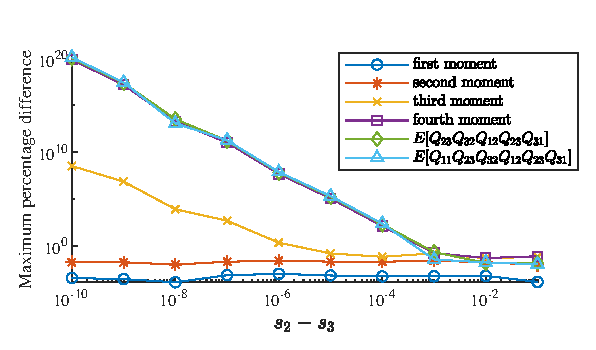
\includegraphics[scale=1.4]{figures/MF-moment-error-degenerate}
	\caption[Maximum difference between Monte Carlo method and the proposed recursive calculation when $s_2$ is close to $s_3$ for moments of the matrix Fisher distribution.]{Maximum difference between Monte Carlo method and the proposed recursive calculation when $s_2$ is close to $s_3$, with $s_1=25$, $s_2=10$.
	Double precision floating-point format is used in the recursive calculation. \label{fig:MF-moment-error-degenerate}}
\end{figure}

\section{Highly Concentrated Approximations of Matrix Fisher Distribution} \label{section:MF-approx}

The normalizing constant of the matrix Fisher distribution and its derivatives can be evaluated using the one dimensional integration formulae given in \eqref{eqn:MF-normalizing-1dInt} and $\eqref{eqn:MF-S2D-1dint}$, or using the saddle point approximation as discussed in \cite{gilitschenski2014efficient}.
However, these approaches are very computationally demanding.
Also, to inference the parameters $F$ from random samples, one must solve the partial differential equation in \eqref{eqn:MF-S2D}.
Because $d_i+d_j$ monotonically increases with $s_i+s_j$ for $i\neq j \in \{1,2,3\}$, and $d_i+d_j$ is upper bounded by 2, the average rate of change of $D$ with respect to $S$ becomes very small when $S$ is very large.
This makes \eqref{eqn:MF-S2D} extremely difficult to solve when $S$ has very large values.

However, large $S$ means the matrix Fisher distribution is highly concentrated.
As an analog of Gaussian distribution on $\SO{3}$, it can actually be approximated by a Gaussian distribution when $S$ is large.
This is similar to the von Mises and von Mises--Fisher distributions on $\Sph^n$ \cite{mardia2009directional}.
Nevertheless, since $\SO{3}$ has three degrees of freedom, the number of degrees of freedom in which the distribution is highly concentrated must be specified.
In the subsequent two subsections, the cases when the matrix Fisher distribution is highly concentrated in all three degrees of freedom, and in two degrees of freedom, are discussed.
And these approximations lead to simplifications of the normalizing constant, and its first order derivatives, which are computational costly to be evaluated.
The results can be further used to expedite the MLE of the parameter F, which requires solving the partial differential equation \eqref{eqn:MF-S2D} involving the normalizing constant.
Unfortunately, we were unable to give an approximation when the matrix Fisher distribution is only highly concentrated in one degree of freedom using the same strategy.

\subsection{Highly Concentrated in Three Degrees of Freedom}

As shown in \eqref{eqn:MF-density-principal}, the concentration of a matrix Fisher distribution along the $i$-th principal axis is controlled by $s_j+s_k$ for $i\neq j\neq k$.
Thus $s_1+s_2 \geq s_1+s_3 \geq s_2+s_3$, $s_2+s_3 \gg 0$ implies the distribution is highly concentrated in all three degrees of freedom.
The Gaussian approximation for this case has been studied in \cite{lee2018bayesian-b}, and is reviewed in this subsection.

\begin{theorem}[\cite{lee2018bayesian-b}] \label{thm:MF-approx-1d}
	Let $R\sim\mathcal{M}(F)$, where $F=USV^T$ is the pSVD of $F$.
	Suppose $s_2+s_3\gg 0$.
	Let $Q = U^TRV = \exp\left(\hat{\eta}\right)$, then $\eta \approxsim \mathcal{N}\big( 0,\allowbreak (\tr{S}I_{3\times 3}-S)^{-1} \big)$, where $\approxsim$ denotes ``approximately follows''.
\end{theorem}
\begin{proof}
	Let $\Sigma = (\tr{S}I_{3 \times 3}-S)^{-1} = \diag\left(\frac{1}{s_2+s_3},\frac{1}{s_1+s_3},\frac{1}{s_1+s_2}\right) \in\mathbb{R}^{3\times 3}$, and let $\xi\in\mathbb{R}^3$ be defined as $\sqrt{\Sigma}\xi = \eta$.
	Then the density \eqref{eqn:MF-density} for $R$ can be written as
	\begin{align*}
		&\etr{FR^T} = \etr{S\exp\left( (\sqrt{\Sigma}\xi)^\wedge \right)} \\
		=\; &\etr{S \Big( I_{3\times 3} + (\sqrt{\Sigma}\xi)^\wedge + \tfrac{1}{2} \big((\sqrt{\Sigma}\xi)^\wedge\big)^2 + O(\sqrt{\Sigma}) \Big)} \\
		=\; &\etr{\tfrac{1}{2}S\big((\sqrt{\Sigma}\xi)^\wedge\big)^2 + O(\sqrt{\Sigma})} \\
		\approx\; &\etr{S} \exp\left(-\tfrac{1}{2}\eta^T\Sigma^{-1}\eta\right).
	\end{align*}
	This finishes the proof.
\end{proof}

Theorem \ref{thm:MF-approx-1d} gives the following approximation of the normalizing constant.
\begin{corollary}[\cite{lee2018bayesian-b}] \label{cor:MF-normal-approx1}
	If $s_2+s_3\gg 0$, then
	\begin{align}
		c(S) &\approx \frac{\etr{S}}{\sqrt{8\pi(s_1+s_2)(s_1+s_3)(s_2+s_3)}} \label{eqn:MF-normalizing-approx1} \\
		\frac{1}{c(S)} \frac{\partial c(S)}{\partial s_i} &\approx 1 - \frac{1}{2}\left( \frac{1}{s_i+s_j} + \frac{1}{s_i+s_k} \right), \label{eqn:MF-S2D-approx1}
	\end{align}
	for $i,j,k\in\{1,2,3\}$ and $i\neq j\neq k$.
\end{corollary}
\begin{proof}
	According to \cite[Chapter 12.1.2]{chirikjian2011stochastic}, \eqref{eqn:MF-normalizing} can be written as
	\begin{align*}
		c(S) = \int_{\norm{\eta}<\pi} \etr{S\exp(\hat{\eta})} \frac{1-\cos\norm{\eta}}{4\pi^2\norm{\eta}^2} \diff\eta,
	\end{align*}
	where $\diff\eta$ is the Lebesgue measure on $\mathbb{R}^3$.
	Using the calculation in Theorem \ref{thm:MF-approx-1d}, and the Taylor expansion of $1-\cos x$, it can further be calculated as
	\begin{align*}
		c(S) &= \etr{S} \int_{\norm{\eta}<\pi} \expb{-\tfrac{1}{2} \eta^T \Sigma^{-1} \eta + O(\sqrt{\Sigma})} (1+O(\Sigma)) \tfrac{1}{8\pi^2} \diff\eta \\
		&\approx \int_{\mathbb{R}^3} \expb{-\tfrac{1}{2} \eta^T \Sigma^{-1} \eta}  \tfrac{1}{8\pi^2} \diff\eta.
	\end{align*}
	Then \eqref{eqn:MF-normalizing-approx1} can be obtained using the normalizing constant of $\mathcal{N}(0,\Sigma)$, and its derivation can also be calculated directly as \eqref{eqn:MF-S2D-approx1}.
\end{proof}

\begin{figure}
	\centering
	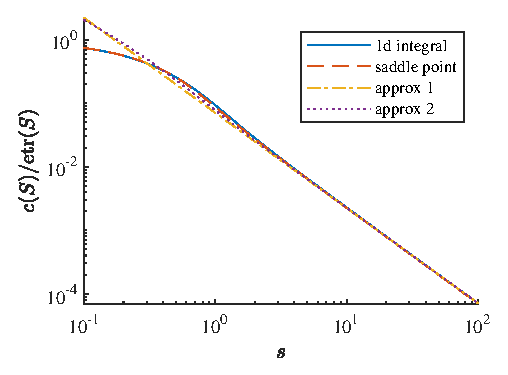
\includegraphics[scale=1.4]{figures/MF-normal-approx1}
	\caption[Comparison of the normalizing constant $c(S)$ calculated using different methods.]{Comparison of the normalizing constant $c(S)$ calculated using the one dimensional integral formula \eqref{eqn:MF-normalizing-1dInt}, the saddle point approximation \cite{kume2005saddlepoint}, the highly concentrated approximations \eqref{eqn:MF-normalizing-approx1} (approx 1) and \eqref{eqn:MF-normalizing-approx2} (approx 2).
	The parameter is $S = sI_{3\times 3}$.
	\label{fig:MF-nomral-approx1}}
\end{figure}

\begin{figure}
	\centering
	\includegraphics[scale=1.4]{figures/MF-S2D-approx1}
	\caption[Comparison of the first order moment $1-d_1$ calculated using different methods.]{Comparison of the first order moment $1-d_1$ calculated using the one dimensional integral formula \eqref{eqn:MF-S2D-1dint}, the saddle point approximation \cite{kume2005saddlepoint,kume2007derivatives}, the highly concentrated approximations \eqref{eqn:MF-S2D-approx1} (approx 1) and \eqref{eqn:MF-S2D-approx2-1} (approx 2).
	The parameter is $S = sI_{3\times 3}$.
	\label{fig:MF-S2D-approx1}}
\end{figure}

Corollary \ref{cor:MF-normal-approx1} provides a very fast computation for the normalizing constant $c(S)$ and its first order derivatives, using only basic functions.
Its accuracy is demonstrated in Figure \ref{fig:MF-nomral-approx1} against the one dimensional integral formula \eqref{eqn:MF-S2D-1dint}, and the saddle point approximation in \cite{kume2005saddlepoint}.
In addition, since the case when the matrix Fisher distribution is highly concentrated in two dimensions is a special case when it is highly concentrated in all three dimensions, the approximation in \eqref{eqn:MF-normalizing-approx2} is also compared.
The tested parameter is when $S = sI_{3\times 3}$, for $s$ ranging from 0.1 to 100.
It is shown that all calculations agree well when $s > 50$, whereas when $s < 50$, the two approximations deviate from the other two calculations, due to that the distribution is no longer highly concentrated.

The derivative of $c(S)$ is compared as $1-d_1 = 1-\tfrac{1}{c(S)} \tfrac{\partial c(S)}{\partial s_1}$ in Figure \ref{fig:MF-S2D-approx1}.
Again, all calculates are very close when $s>10$, but the two approximations become less accurate when the distribution is not highly concentrated.
It should be note that for extremely large $s$, for example when $s > 10^4$, the one dimensional integral formula, especially for the derivative \ref{eqn:MF-S2D-1dint}, becomes inaccurate when implemented with MATLAB \texttt{integral} function.

\subsection{Highly Concentrated in Two Degrees of Freedom} \label{section:MF-approx-2}

In this subsection, the case when $s_1+s_3\gg s_2+s_3 \geq 0$ is considered, i.e., the matrix Fisher distribution is highly concentrated along the second and third principal axes, but has large dispersion along the first axis.
Note that because $s_1 \geq s_2 \geq |s_3| \geq 0$, $s_1+s_3\gg s_2+s_3$ is equivalent to $s_1 \gg s_2$.
It is proved in this case, the matrix Fisher distribution can be approximated by a combination of a two dimensional Gaussian distribution in $\mathbb{R}^2$, and a one dimensional von Mises distribution on $\Sph^1$.

\begin{theorem} \label{thm:MF-approx-2d}
	Let $R\sim\mathcal{M}(F)$, where $F=USV^T$ is the pSVD of $F$.
	Suppose $s_1+s_3\gg 0$.
	Let $Q = U^TRV = \exp\left(\hat{\eta}\right) \exp\left(\hat{\eta}'\right)$, where $\eta = [0, \eta_2, \eta_3]^T$, and $\eta' = [\eta_1, 0, 0]^T$.
	Then $\eta_3 \approxsim \mathcal{VM}(0,s_2+s_3)$, and $ [\eta_2, \eta_3]^T  \approxsim \mathcal{N}\left( 0, \diag\left( \tfrac{1}{s_1+s_3}, \tfrac{1}{s_1+s_2} \right) \right)$, and they are approximately independent.
\end{theorem}
\begin{proof}
	let $\Sigma = \diag\left( 0, \tfrac{1}{s_1+s_3}, \tfrac{1}{s_1+s_2} \right)$, and $\eta = \sqrt{\Sigma} \xi$.
	Then $\exp\left(\hat{\eta}\right)$ can be written as
	\begin{align*}
		\exp\left(\hat{\eta}\right) = I_{3\times 3} + \sqrt{\Sigma}\hat{\xi} + \tfrac{1}{2} \left( \sqrt{\Sigma}\hat{\xi} \right)^2 + O\big(s_1^{-3/2}\big).
	\end{align*}
	Also, $\exp\left(\hat{\eta}'\right)$ can be explicitly calculated as
	\begin{align*}
		\exp\left(\hat{\eta}'\right) = \begin{bmatrix}
			1 & 0 & 0 \\
			0 & \cos\eta_1 & -\sin\eta_1 \\
			0 & \sin\eta_1 & \cos\eta_1
		\end{bmatrix}.
	\end{align*}
	Combining the above two equations, the density function for $R$ becomes
	\begin{align*}
		\etr{FR^T} &= \etr{S\exp(\hat{\eta})\exp(\hat{\eta}')} \\
		&= \exp(s_1) \cdot \exp((s_2+s_3)\cos\eta_1) \cdot \expb{-\tfrac{1}{2} \left( (s_1+s_3)\eta_2^2 + (s_1+s_2)\eta_3^2 \right)} \\
		&\quad \cdot \expb{-\tfrac{1}{2}\left( (s_2\eta_3^2 + s_3\eta_2^2)(\cos\eta_1-1) + (s_3-s_2)\eta_2\eta_3\sin\eta_1 \right) + O\big(s_1^{-1/2}\big)}.
	\end{align*}
	Note that the last exponential term can be simplified as
	\begin{align*}
		&(s_2\eta_3^2 + s_3\eta_2^2)(\cos\eta_1-1) + (s_3-s_2)\eta_2\eta_3\sin\eta_1 \\
		= &\left( \tfrac{s_2}{s_1+s_2}\xi_3^2 + \tfrac{s_3}{s_1+s_3}\xi_2^2 \right)(\cos\eta_1-1) + \tfrac{s_3-s_2}{\sqrt{s_1+s_3} \sqrt{s_1+s_2}} \xi_2\xi_3 \sin\eta_1 \\
		= & O\big(s_1^{-1}\big).
	\end{align*}
	So the density function for $R$ can be approximated by
	\begin{align*}
		\etr{FR^T} \approx \exp(s_1) \cdot \exp((s_2+s_3)\cos\eta_1) \cdot \expb{-\tfrac{1}{2} \left( (s_1+s_3)\eta_2^2 + (s_1+s_2)\eta_3^2 \right)},
	\end{align*}
	and the desired result is proved.
\end{proof}

Before looking into how this approximation can be applied to calculating the normalizing constant $c(S)$, a decomposition of the Haar measure $\diff Q$ on $\SO{3}$ needs to be introduced first \cite[Chapter 4]{dym1972fourier}.
Let $\mathbf{K} = \{\expb{\theta\hat{e}_1} \,|\, 0\leq \theta < 2\pi\}$ be a subgroup of $\SO{3}$, it is clear that $\mathbf{K}$ is isomorphic to $\SO{2} \cong \Sph^1$.
The quotient group of $\mathbf{K}$ is $\SO{3}/\mathbf{K} = \{ T\in\SO{3} \,|\, T\mathbf{K} \}$, which is isomorphic to $\Sph^2$ under the map
\begin{align} \label{eqn:SO3-SO3/K}
	j:\, \SO{3}/\mathbf{K} \to \Sph^2, \qquad T\mathbf{K} \mapsto Te_1.
\end{align}
Therefore, for any $Q\in\SO{3} = \SO{3}/\mathbf{K} \times \mathbf{K} \cong \Sph^2\times \Sph^1$, it can be decomposed as $Q = T(x) \expb{\theta\hat{e}_1}$,
for $x\in\Sph^2$ and $0\leq \theta< 2\pi$, where $T\mathbf{K} = j^{-1}(x)$.
And the Haar measure $\diff{Q}$ can be decomposed as $\tfrac{1}{8\pi^2} \diff \theta \diff \sigma(x)$, where $\diff \sigma(x)$ is the surface area measure on $\Sph^2$.
This decomposition can be used to obtain an approximation of the normalizing constant given in the next Corollary.

\begin{corollary}
	If $s_1+s_3 \gg s_2+s_3$, then
	\begin{align}
		c(S) &\approx \frac{\exp(s_1)I_0(s_2+s_3)}{2\sqrt{(s_1+s_2)(s_1+s_3)}}, \label{eqn:MF-normalizing-approx2} \\
		\frac{1}{c(S)}\frac{\partial c(S)}{\partial s_1} &\approx 1 - \frac{1}{2}\left( \frac{1}{s_1+s_2} + \frac{1}{s_1+s_3} \right), \label{eqn:MF-S2D-approx2-1} \\
		\frac{1}{c(S)}\frac{\partial c(S)}{\partial s_j} &\approx \frac{I_1(s_2+s_3)}{I_0(s_2+s_3)} - \frac{1}{2}\frac{1}{s_1+s_j}, \label{eqn:MF-S2D-approx2-2}
	\end{align}
	for $j\in\{2,3\}$.
\end{corollary}
\begin{proof}
	As shown in Theorem \ref{thm:MF-approx-2d}, $c(S)$ can be calculated as
	\begin{align*}
		c(S) \approx \exp(s_1) \int_{Q\in\SO{3}} \exp((s_2+s_3)\cos\eta_1) \cdot \expb{-\tfrac{1}{2} \left( (s_1+s_3)\eta_2^2 + (s_1+s_2)\eta_3^2 \right)} \diff Q
	\end{align*}
	Let $x = [\cos\alpha, \sin\alpha\cos\beta, \sin\alpha\sin\beta]^T \in \Sph^2$ be written in spherical coordinates, then using \eqref{eqn:SO3-SO3/K}, it can be shown that $j^{-1}(x) = \expb{\hat{\eta}} \mathbf{K}$, if $\eta$ is re-parameterized in polar coordinates as $\eta_2 = -\alpha\sin\beta$, $\eta_3 = \alpha\cos\beta$.
	Thus, $c(S)$ can be written as
	\begin{align*}
		c(S) &\approx \exp(s_1) \int_{0}^{2\pi} \exp((s_2+s_3)\cos\eta_1) \frac{1}{2\pi} \diff \eta_1 \\
		&\qquad \cdot \int_{0}^\pi \int_{0}^{2\pi} \expb{-\tfrac{1}{2} \left( (s_1+s_3)\eta_2^2 + (s_1+s_2)\eta_3^2 \right)} \frac{1}{4\pi} \sin\alpha \diff\beta \diff\alpha,
	\end{align*}
	where the first integral term is the normalizing constant of the von Mises distribution \cite[Chapter 3]{mardia2009directional}, given by $I_0(s_2+s_3)$.
	Note that $\eta_2 = \tfrac{\xi_2}{\sqrt{s_1+s_3}}$, and $\eta_3 = \tfrac{\xi_3}{\sqrt{s_1+s_2}}$, so $\sin\alpha = \alpha + O(s_1^{-3/2})$. Also, the integration for $\expb{-\tfrac{1}{2} \left( (s_1+s_3)\eta_2^2 + (s_1+s_2)\eta_3^2 \right)}$ becomes very small for $\alpha > \pi$ as $s_1+s_3 \gg 0$.
	Therefore, the second integral can be approximated by
	\begin{align*}
		&\int_0^\infty \int_{0}^{2\pi} \expb{-\tfrac{1}{2} \left( (s_1+s_3)\eta_2^2 + (s_1+s_2)\eta_3^2 \right)} \frac{1}{4\pi} \alpha \diff\beta \diff\alpha \\
		= &\int_{-\infty}^\infty \int_{-\infty}^\infty \expb{-\tfrac{1}{2} \left( (s_1+s_3)\eta_2^2 + (s_1+s_2)\eta_3^2 \right)} \frac{1}{4\pi} \diff\eta_2 \diff\eta_3,
	\end{align*}
	which is the normalizing constant of the Gaussian distribution.
	And \eqref{eqn:MF-normalizing-approx2} follows after combining the two integral terms.
	The derivatives \eqref{eqn:MF-S2D-approx2-1} and \eqref{eqn:MF-S2D-approx2-2} can be directly calculated by differentiating \eqref{eqn:MF-normalizing-approx2}.
\end{proof}

\begin{figure}
	\centering
	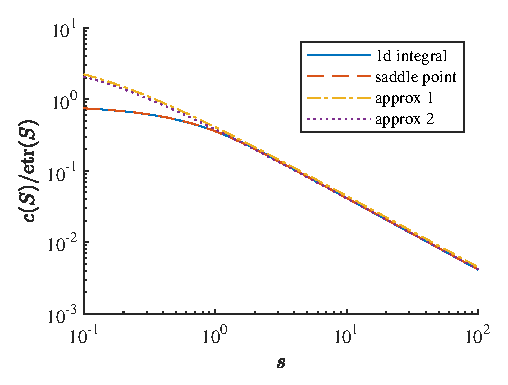
\includegraphics[scale=1.4]{figures/MF-normal-approx2}
	\caption[Comparison of the normalizing constant $c(S)$ calculated using different methods.]{Comparison of the normalizing constant $c(S)$ calculated using the one dimensional integral formula \eqref{eqn:MF-normalizing-1dInt}, the saddle point approximation \cite{kume2005saddlepoint}, the highly concentrated approximations \eqref{eqn:MF-normalizing-approx1} (approx 1) and \eqref{eqn:MF-normalizing-approx2} (approx 2).
	The parameter is $S = \diag(s,0.1,0.1)$.
	\label{fig:MF-nomral-approx2}}
\end{figure}

\begin{figure}
	\centering
	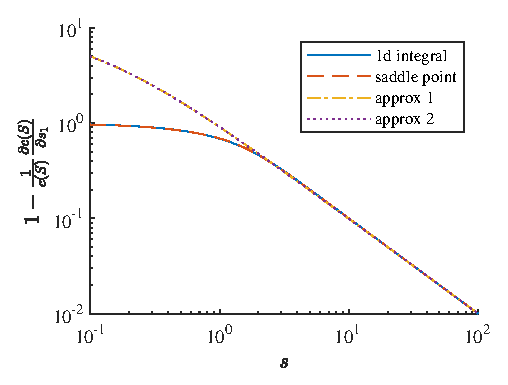
\includegraphics[scale=1.4]{figures/MF-S2D-approx2-1}
	\caption[Comparison of the first order moment $1-d_1$ calculated using different methods.]{Comparison of the first order moment $1-d_1$ calculated using the one dimensional integral formula \eqref{eqn:MF-S2D-1dint}, the saddle point approximation \cite{kume2005saddlepoint,kume2007derivatives}, the highly concentrated approximations \eqref{eqn:MF-S2D-approx1} (approx 1) and \eqref{eqn:MF-S2D-approx2-1} (approx 2).
	The parameter is $S = \diag(s,0.1,0.1)$.
	\label{fig:MF-S2D-approx2-1}}
\end{figure}

\begin{figure}
	\centering
	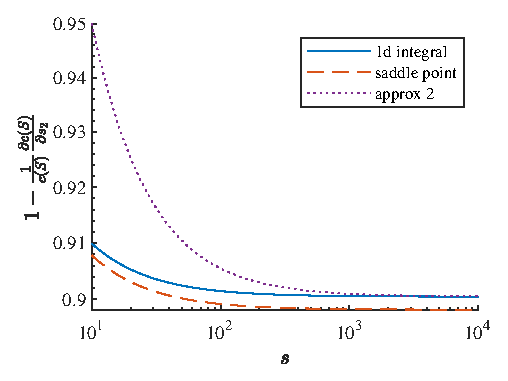
\includegraphics[scale=1.4]{figures/MF-S2D-approx2-2}
	\caption[Comparison of the first order moment $1-d_2$ calculated using different methods.]{Comparison of the first order moment $1-d_2$ calculated using the one dimensional integral formula \eqref{eqn:MF-S2D-1dint}, the saddle point approximation \cite{kume2005saddlepoint,kume2007derivatives}, the highly concentrated approximations \eqref{eqn:MF-S2D-approx2-2} (approx 2).
	The parameter is $S = \diag(s,0.1,0.1)$.
	\label{fig:MF-S2D-approx2-2}}
\end{figure}

Although the approximations \eqref{eqn:MF-normalizing-approx2} and \eqref{eqn:MF-S2D-approx2-2} involve the modified Bessel function of the first kind, then are much easier to be evaluated than $c(S)$ itself.
The comparision of $c(S)$ calculated from different methods is shown in Figure \ref{fig:MF-nomral-approx2}, for $S = \diag(s,0.1,0.1)$ with $s$ rangin from 0.1 to 100.
It can be seen that when $s>50$, the approximation \eqref{eqn:MF-normalizing-approx2} is very close to the one dimensional integral and saddle point approximation.
However, because $s_2+s_3 = 0.2$ is very small, the matrix Fisher distribution has very large dispersion in the first principal axis, and the approximation \eqref{eqn:MF-normalizing-approx1} developed for high concentration in all three degrees of freedom does not approximate $c(S)$ as well as \eqref{eqn:MF-normalizing-approx2}, even when $s_1 = s$ is large.

Next, the comparison of $1-d_1 = 1-\tfrac{1}{c(S)} \tfrac{\partial c(S)}{\partial s_1}$ is presented in Figure \ref{fig:MF-S2D-approx2-1}.
Similarly, the approximation \eqref{eqn:MF-S2D-approx2-1} becomes very close to the one dimensional integral and saddle point approximation.
And since \eqref{eqn:MF-S2D-approx1} is the same as \eqref{eqn:MF-S2D-approx2-1}, it also approximates the derivative well.
The comparison of $1-d_2 = 1-\tfrac{1}{c(s)}\tfrac{\partial c(S)}{\partial s_2}$ is presented in Figure \ref{fig:MF-S2D-approx2-2} for $S = \diag(s,0.1,0.1)$ with $s$ ranging from 10 to 10000.
It can be seen that the difference between the approximation \eqref{eqn:MF-S2D-approx2-2} and one dimensional integral becomes small when $s>500$.
The approximation \eqref{eqn:MF-S2D-approx1} for high concentration in all three degrees of freedom is not shown because its error is too large.
Also, it appears the that one dimensional integral is more accurate than the saddle point approximation, which is in general the case for $S$ that are not extremely large.

In summary, this chapter reviews the matrix Fisher and Bingham distributions that are used to model large uncertainty of 3D attitude.
A recursive algorithm is derived to calculate the central moments of the matrix Fisher distribution up to an arbitrary order.
Also, an approximation is proposed when the matrix Fisher distribution is highly concentrated in two degrees of freedom, which is used to derive simplified expressions for the normalizing constant and its derivatives.

% !TEX root = ../thesis-WW.tex

\chapter{Matrix Fisher-Gaussian Distribution} \label{chap:MFG}



% !TEX root = ../thesis-WW.tex

\chapter{Bayesian Estimation with Matrix Fisher-Gaussian Distribution} \label{chap:estimation}











\bibliographystyle{plain}
\bibliography{thesis-bib}

% appendices must appear after
% !TEX root = ../thesis-WW.tex
\appendix
\doublespacing

\chapter{A Special Case in Theorem \ref{thm:MF-moment-dsdT}} \label{app:MF-moment-specialRecursion}

In this supplementary material, a special case which is embedded in the recursion of Theorem \eqref{thm:MF-moment-dsdT} is untwisted into a non-recursive formula except for an integer coefficient.

\begin{theorem} \label{thm:MF-moment-specialRecursion}
	If $s_1 \neq s_2 \neq |s_3|$ and $i \neq j$, then
	\begin{align} \label{eqn:dsisjdT}
		\left.\left( \frac{\partial^{2n}s'_i}{\partial T_{ij}^{2n}} + \frac{\partial^{2n}s'_j}{\partial T_{ij}^{2n}} \right)\right|_{T=0} &= \frac{a(n)}{(s_i+s_j)^{2n-1}}, \nonumber \\
		\left.\left( \frac{\partial^{2n}s'_i}{\partial T_{ij}^{2n}} - \frac{\partial^{2n}s'_j}{\partial T_{ij}^{2n}} \right)\right|_{T=0} &= \frac{a(n)}{(s_i-s_j)^{2n-1}},
	\end{align}
	where $a(n)$ is an integer-valued function of $n$.
\end{theorem}

Before proving this theorem, a lemma for differentiating $U'$ and $V'$ is needed.
\begin{lemma} \label{lemma:MF-moment-dUVdT-zero}
	Under the conditions of Theorem \ref{thm:MF-moment-dsdT}, if any of $k$ or $l$ is distinct from $i$ or $j$, then
	\begin{equation}
		\left. \frac{\partial^n U'_{kl}}{\partial T_{ij}^n} \right|_{T=0} = 0, \qquad
		\left. \frac{\partial^n V'_{kl}}{\partial T_{ij}^n} \right|_{T=0} = 0,
	\end{equation}
	for all $n>0$.
\end{lemma}
\begin{proof}
	Suppose $i=1,j=2$, and let $\begin{bmatrix} s_1 & T_{12} \\ 0 & s_2 \end{bmatrix} = \begin{bmatrix} U'_{11} & U'_{12} \\ U'_{21} & U'_{22} \end{bmatrix} \begin{bmatrix} s'_1 & 0 \\ 0 & s'_2 \end{bmatrix} \begin{bmatrix} V'_{11} & V'_{12} \\ V'_{21} & V'_{22} \end{bmatrix}^T$ be the singular value decomposition of the upper left 2-by-2 diagonal block of $S+T$.
	Then by direct calculation, $S+T$ has singular value decomposition
	\begin{equation*}
		\begin{bmatrix}
			s_1 & T_{12} & 0 \\
			0 & s_2 & 0 \\
			0 & 0 & s_3
		\end{bmatrix} = \begin{bmatrix}
			U'_{11} & U'_{12} & 0 \\
			U'_{21} & U'_{22} & 0 \\
			0 & 0 & 1
		\end{bmatrix} \begin{bmatrix}
			s'_1 & 0 & 0 \\
			0 & s'_2 & 0 \\
			0 & 0 & s_3
		\end{bmatrix} \begin{bmatrix}
			V'_{11} & V'_{12} & 0 \\
			V'_{21} & V'_{22} & 0 \\
			0 & 0 & 1
		\end{bmatrix}^T.
	\end{equation*}
	This means if the subscripts of $U'$ or $V'$ contain $3$ which is different from $\{1,2\}$, the corresponding element of $U'$ or $V'$ is either zero or one, whose derivatives with respect to $T_{12}$ of any order evaluated at $T=0$ is zero.
	Other cases can be shown similarly.
\end{proof}

Next, the proof for Theorem \ref{thm:MF-moment-specialRecursion} is provided.
\begin{proof}
	By direct calculation using \eqref{eqn:dsvd-dsdT}, is can be shown that
	\begin{align*}
		\frac{\partial (s'_i+s'_j)}{\partial T_{ij}} &= U'_{ii}V'_{ji} + U'_{ij}V'_{jj} \triangleq X_1, \\
		\frac{\partial (s'_i-s'_j)}{\partial T_{ij}} &= U'_{ii}V'_{ji} - U'_{ij}V'_{jj} \triangleq X_2,
	\end{align*}
	for $X_1,X_2\in\mathbb{R}$.
	Next, the second order differentiation is calculated using \eqref{eqn:dsvd-dUVdT} as
	\begin{align*}
		\frac{\partial X_1}{\partial T_{ij}}
		&= (U'_{ii}V'_{jj}-U'_{ij}V'_{ji})(\Omega_{U_{ij}}^{ij}+\Omega_{V_{ij}}^{ij}) + U'_{ik}V'_{ji}\Omega_{U_{ki}}^{ij} - U'_{ii}V'_{jk}\Omega_{V_{ki}}^{ij} + U'_{ik}V'_{jj}\Omega_{U_{kj}}^{ij} - U'_{ij}V'_{jk}\Omega_{V_{kj}}^{ij}, \\
		\frac{\partial X_2}{\partial T_{ij}} &= (U'_{ii}V'_{jj}+U'_{ij}V'_{ji})(\Omega_{V_{ij}}^{ij}-\Omega_{U_{ij}}^{ij}) + U'_{ik}V'_{ji}\Omega_{U_{ki}}^{ij} - U'_{ii}V'_{jk}\Omega_{V_{ki}}^{ij} - U'_{ik}V'_{jj}\Omega_{U_{kj}}^{ij} + U'_{ij}V'_{jk}\Omega_{V_{kj}}^{ij},
	\end{align*}
	where $k\in\{1,2,3\}$ and $i\neq j\neq k$.
	The crucial observation is that if we further differentiate the above two equations with respect to $T_{ij}$ and evaluate at $T=0$, then the last four terms in each subequation yield terms involving either $U'_{ik}$, $V'_{jk}$, or their derivatives with respect to $T_{ij}$.
	However, Lemma \ref{lemma:MF-moment-dUVdT-zero} indicates that all these terms vanish after evaluated at $T=0$.
	This means when calculating \eqref{eqn:dsisjdT}, the last four terms in each of the above subequations can be simply omitted.
	Therefore, by \eqref{eqn:dsvd-OmegaUV} is can be shown that
	\begin{align*}
		\frac{\partial X_1}{\partial T_{ij}} &= (U'_{ii}V'_{jj}-U'_{ij}V'_{ji})(\Omega_{U_{ij}}^{ij}+\Omega_{V_{ij}}^{ij}) = \frac{(U'_{ii}V'_{jj}-U'_{ij}V'_{ji})^2}{s'_i+s'_j} \triangleq \frac{Y_1^2}{s'_i+s'_j}, \\
		\frac{\partial X_2}{\partial T_{ij}} &= (U'_{ii}V'_{jj}+U'_{ij}V'_{ji})(-\Omega_{U_{ij}}^{ij}+\Omega_{V_{ij}}^{ij}) = \frac{(U'_{ii}V'_{jj}+U'_{ij}V'_{ji})^2}{s'_i-s'_j} \triangleq \frac{Y_2^2}{s'_i-s'_j}.
	\end{align*}
	If the above two equations are differentiated with respect to $T_{ij}$ again, we obtain the derivatives of $s_i \pm s_j$ which have been calculated, and the derivatives of $Y_1$, $Y_2$ which are calculated as follows.
	\begin{align*}
		\frac{\partial Y_1}{\partial T_{ij}} &= -\frac{(V'_{ii}V'_{ji}+U'_{ij}V'_{jj})(U'_{ii}V'_{jj}-U'_{ij}V'_{ji})}{s'_i+s'_j} = -\frac{X_1Y_1}{s'_i+s'_j}, \\
		\frac{\partial Y_2}{\partial T_{ij}} &= -\frac{(U'_{ii}V'_{ji}-U'_{ij}V'_{ji})(U'_{ii}V'_{jj}+U'_{ij}V'_{ji})}{s'_i-s'_j} = -\frac{X_2Y_2}{s'_i-s'_j},
	\end{align*}
	where any term having the subscript $k$ has been omitted. 
	
	Now, a very special branch of smaller recursion is distilled from the large recursion stated in Theorem \ref{thm:MF-moment-dsdT}, which reads
	\begin{align} \label{eqn:smallRecursion}
		\frac{\partial (s'_i+s'_j)}{\partial T_{ij}} &= X_1, \qquad \frac{\partial X_1}{\partial T_{ij}} = \frac{Y_1^2}{s'_i+s'_j}, \qquad \frac{\partial Y_1}{\partial T_{ij}} = -\frac{X_1Y_1}{s'_i+s'_j}, \nonumber \\
		\frac{\partial (s'_i-s'_j)}{\partial T_{ij}} &= X_2, \qquad \frac{\partial X_2}{\partial T_{ij}} = \frac{Y_2^2}{s'_i-s'_j}, \qquad \frac{\partial Y_2}{\partial T_{ij}} = -\frac{X_2Y_2}{s'_i-s'_j}.
	\end{align}
	Since the recursive structure for $s'_i+s'_j$ and $s'_i-s'_j$ are the same, they can be written in the same form as
	\begin{equation*}
		\frac{\partial s'_{ij}}{\partial T_{ij}} = X; \qquad \frac{\partial X}{\partial T_{ij}} = \frac{Y^2}{s'_{ij}}; \qquad \frac{\partial Y}{\partial T_{ij}} = -\frac{XY}{s'_{ij}},
	\end{equation*}
	where $s'_{ij}$ denotes either $s'_i+s'_j$ or $s'_i-s'_j$.
	Finally, to prove the theorem, it is claimed that
	\begin{equation*}
		\frac{\partial^{2n} s'_{ij}}{\partial T_{ij}^{2n}} = \frac{a_0Y^{2n} + a_1Y^{2n-2}X^2 + \cdots + a_{n-1}Y^2X^{2n-2}}{{s'_{ij}}^{2n-1}},
	\end{equation*}
	where $a_m$ is an integer coefficient for $m=0,\ldots,n-1$.
	This claim is proved by induction.
	When $n=1$, it is clearly seen from \eqref{eqn:smallRecursion}.
	Suppose for case $n$ it is true, then differentiate $T_{ij}$ one more time, and after some rearrangement, it is shown that
	\begin{equation*}
		\frac{\partial^{2n+1} s'_{ij}}{\partial T_{ij}^{2n+1}} = \frac{a'_0Y^{2n}X + a'_1Y^{2n-2}X^3 + \cdots + a'_{n-1}Y^2X^{2n-1}}{\partial {s'_{ij}}^{2n}},
	\end{equation*}
	where $a'_m = (-4n+2m+1)a_m + 2(m+1)a_{m+1}$ for $m=0,\ldots,n-2$, and $a'_{n-1} = (-2n-1)a_{n-1}$.
	Then, differentiate $T_{ij}$ once again, it is shown that
	\begin{align*}
		\frac{\partial^{2n+2} s'_{ij}}{\partial T_{ij}^{2n+2}} = \frac{a''_0Y^{2n+2} + a''_1Y^{2n}X^2 + \cdots + a''_{n}Y^2X^{2n}}{{s'_{ij}}^{2n+1}},
	\end{align*}
	where $a''_0 = a'_0$, $a''_m = (-4n+2m-2)a'_{m-1} + (2m+1)a'_m$ for $m=1,\ldots,n-1$, and $a''_n = (-2n-2)a'_{n-1}$.
	This finishes the proof for the claim.
	Now, note that when evaluated at $T=0$, we have $Y=1$, $X=0$.
	Thus $\left. \partial^{2n}s'_{ij} / \partial T_{ij}^{2n} \right|_{T=0} = a_0 / s_{ij}^{2n-1}$, which finishes the proof for Theorem \ref{thm:MF-moment-specialRecursion} by noting that $a_0$ is an integer function of $n$.
\end{proof}

It should be noted that the idea in the proof of Theorem \ref{thm:MF-moment-specialRecursion} cannot be generalized to the large recursion stated in Theorem \ref{thm:MF-moment-dsdT}, due to the omitted terms in the derivatives of $X$ and $Y$.
Even in this simpler case, giving a non-recursive expression for $a(n)$ is complicated, as seen from the recursive formula given for $a_m(n)$ in the proof.

\chapter{The Second and Third Order Moment of Matrix Fisher Distribution} \label{app:MF-moment-second-third}

In this Appendix, non-recursive expressions of the second and third order moments are provided based on the development in Chapter \ref{section:MF-moments}.

\section{The Second Order Moments}

Based on Lemma \ref{lemma:MF-moment-EQii}, the second order moment of the form $\expect{Q_{ii}Q_{jj}}$ can be calculated as
\begin{align} \label{eqn:MF-moment-EQiijj}
	\expect{Q_{ii}Q_{jj}} = \frac{1}{c(S)} \frac{\partial^2 c(S)}{\partial s_i \partial s_j},
\end{align}
for any $i,j\in\{1,2,3\}$.
Next, using the recursion developed in Theorem \ref{thm:MF-moment-dsdT}, the second order moment of the forms $\expect{Q_{ij}Q_{ij}}$ and $\expect{Q_{ij}Q_{ji}}$ can be calculated as
\begin{subequations} \label{eqn:MF-moment-EQijij-EQijji}
	\begin{align}
		\expect{Q_{ij}Q_{ij}} &= \frac{1}{c(S)}\left(-\frac{\partial c(S)}{\partial s_i}\frac{s_i}{s_j^2-s_i^2}+\frac{\partial c(S)}{\partial s_j}\frac{s_j}{s_j^2-s_i^2}\right), \\
		\expect{Q_{ij}Q_{ji}} &= \frac{1}{c(S)}\left(-\frac{\partial c(S)}{\partial s_i}\frac{s_j}{s_j^2-s_i^2}+\frac{\partial c(S)}{\partial s_j}\frac{s_i}{s_j^2-s_i^2}\right),
	\end{align}
\end{subequations}
for any $i\neq j \in \{1,2,3\}$, and $|s_i|\neq |s_j|$.

If $s_i = s_j \neq 0$, \eqref{eqn:MF-moment-EQijij-EQijji} can be evaluated by taking the limit $s_j\to s_i$, and their explicit expressions are
\begin{subequations} \label{eqn:MF-moment-EQijij-EQijji-degenerate1}
	\begin{align}
		\expect{Q_{ij}Q_{ij}} &= \frac{1}{c(S)}\frac{1}{2s_i} \left( \frac{\partial c(S)}{\partial s_i} + s_i\left( \frac{\partial^2 c(S)}{\partial s_i^2} - \frac{\partial^2 c(S)}{\partial s_i \partial s_j} \right) \right), \\
		\expect{Q_{ij}Q_{ji}} &= \frac{1}{c(S)}\frac{1}{2s_i}\left( -\frac{\partial c(S)}{s_i} + s_i\left( \frac{\partial^2 c(S)}{\partial s_i^2} - \frac{\partial^2 c(S)}{\partial s_i \partial s_j} \right) \right).
	\end{align}
\end{subequations}
Similarly, if $s_i = -s_j \neq 0$, their expressions become
\begin{subequations}
	\begin{align}
		\expect{Q_{ij}Q_{ij}} &= \frac{1}{c(S)} \frac{1}{2s_i} \left( \frac{\partial c(S)}{\partial s_i}  + s_i\left( \frac{\partial^2 c(S)}{\partial s_i^2} + \frac{\partial^2 c(S)}{\partial s_i \partial s_j} \right) \right), \\
		\expect{Q_{ij}Q_{ji}} &= \frac{1}{c(S)} \frac{1}{2s_i} \left( \frac{\partial c(S)}{\partial s_i} - s_i\left( \frac{\partial^2 c(S)}{\partial s_i^2} + \frac{\partial^2 c(S)}{\partial s_i \partial s_j} \right) \right).
	\end{align}
\end{subequations}
If $s_i = s_j = 0$, the above equations can also be evaluated by taking the limit $s_i\to 0$, as
\begin{subequations} \label{eqn:MF-moment-EQijij-EQijji-degenerate3}
	\begin{align}
		\expect{Q_{ij}Q_{ij}} &= \frac{1}{c(S)} \frac{\partial^2 c(S)}{\partial s_i^2}, \\
		\expect{Q_{ij}Q_{ji}} &= -\frac{1}{c(S)} \frac{\partial^2 c(S)}{\partial s_i \partial s_j}.
	\end{align}
\end{subequations}

Given these results and Theorem \ref{thm:MF-moment-dcds}, the second order derivatives of the normalizing constant can be easily evaluated by solving a linear system using the first order derivatives.
This result is summarized in the following theorem.
\begin{theorem} \label{thm:MF-moment-dcds-second}
	Let $\partial^2 c(S) \in \mathbb{R}^{3\times 3}$ be a matrix whose elements are the second order derivatives $\partial^2 c(S)/\partial s_i \partial s_j$, $i,j\in\{1,2,3\}$.
	Then $\partial^2 c(S)$ satisfies a linear system $A \cdot \mathrm{vec}(\partial^2 c(S)) = b$, where $A\in\mathbb{R}^{9\times 9}$ is constant, and $b\in\mathbb{R}^9$ only involves $S$, $c(S)$, and the first order derivatives of $c(S)$.
\end{theorem}
\begin{proof}
	According to \eqref{eqn:MF-moment-EQiijj}, it can be shown that
	\begin{align*}
		\frac{\partial^2 c(S)}{\partial s_i^2} = c(S)\expect{Q_{ii}^2} = c(S)\left(1-\expect{Q_{ij}^2}-\expect{Q_{ik}^2}\right),
	\end{align*}
	where $i\neq j\neq k$.
	If $s_j\neq s_k$, then by \eqref{eqn:MF-moment-EQijij-EQijji} and the above equation, $\partial^2 c(S)/\partial s_i^2$ can be written as an expression involved with $S$, $c(S)$, and the first order derivatives of $c(S)$.
	If $s_j=s_k\neq 0$, or $s_j=-s_k\neq 0$, or $s_j=s_k=0$, substitute \eqref{eqn:MF-moment-EQijij-EQijji-degenerate1} to \eqref{eqn:MF-moment-EQijij-EQijji-degenerate3} into the above equation.
	Then the coefficient of $\partial^2 c(S)/\partial s_i^2$, $\partial^2 c(S)/\partial s_i \partial s_j$, and $\partial^2 c(S)/\partial s_i \partial s_k$ on the right hand side are constants.
	After moving them to the left hand side, the right hand side only has $S$, $c(S)$, and the first order derivatives of $c(S)$.
	These provides three equations in total.
	
	Next, by \eqref{eqn:MF-moment-EQiijj} and \eqref{eqn:SO3-Rkk}, it can be shown that
	\begin{align*}
		\frac{\partial^2 c(S)}{\partial s_i \partial s_j} = c(S)\expect{Q_{ii}Q_{kk}} = c(S)\left(\expect{Q_{kk}}+\expect{Q_{ij}Q_{ji}}\right),
	\end{align*}
	for $i\neq j\neq k$.
	Substitute \eqref{eqn:MF-S2D} and one from \eqref{eqn:MF-moment-EQijij-EQijji} to \eqref{eqn:MF-moment-EQijij-EQijji-degenerate3} into the above equation, and move $\partial^2 c(S)/\partial s_i^2$, $\partial^2 c(S)/\partial s_i \partial s_j$ from the right had side to the left hand side, the remaining six equations are obtained.
\end{proof}

\section{The Third Order Moments}

Based on Lemma \ref{lemma:MF-moment-EQii}, the third order moments of the form
$\expect{Q_{ii}Q_{jj}Q_{kk}}$ are
\begin{align}
	\expect{Q_{ii}Q_{jj}Q_{kk}} = \frac{1}{c(S)} \frac{\partial^3 c(S)}{\partial s_i \partial s_j \partial s_k},
\end{align}
for $i,j,k\in\{1,2,3\}$.
Next, moments of the form $\expect{Q_{ii}Q_{jk}Q_{kj}}$ are
\begin{subequations}
	\begin{align}
		\expect{Q_{ii}Q_{jk}Q_{jk}} &= \frac{1}{c(S)} \left( \frac{\partial^2 c(S)}{\partial s_i \partial s_k} \frac{s_k}{s_k^2-s_j^2} - \frac{\partial^2 c(S)}{\partial s_i \partial s_j} \frac{s_j}{s_k^2-s_j^2} \right), \\
		\expect{Q_{ii}Q_{jk}Q_{kj}} &= \frac{1}{c(S)} \left( \frac{\partial^2 c(S)}{\partial s_i \partial s_k} \frac{s_j}{s_k^2-s_j^2} - \frac{\partial^2 c(S)}{\partial s_i \partial s_j} \frac{s_k}{s_k^2-s_j^2} \right),
	\end{align}
\end{subequations}
for $i\neq j\neq k$ and $|s_j|\neq |s_k|$.
Moments of the form $\expect{Q_{jj}Q_{jk}Q_{jk}}$ are
\begin{subequations}
	\begin{align}
		\expect{Q_{jj}Q_{jk}Q_{jk}} &= \frac{1}{c(S)} \left( \frac{\partial^2 c(S)}{\partial s_j \partial s_k} \frac{s_k}{s_k^2-s_j^2} - \frac{\partial^2 c(S)}{\partial s_j^2} \frac{s_j}{s_k^2-s_j^2} \right. \nonumber \\
		&\qquad\qquad \left. - \frac{\partial c(S)}{\partial s_j} \frac{s_j^2+s_k^2}{(s_j^2-s_k^2)^2} + \frac{\partial c(S)}{\partial s_k} \frac{2s_js_k}{(s_j^2-s_k^2)^2} \right), \\
		\expect{Q_{jj}Q_{jk}Q_{kj}} &= \frac{1}{c(S)} \left( \frac{\partial^2 c(S)}{\partial s_j \partial s_k} \frac{s_j}{s_k^2-s_j^2} - \frac{\partial^2 c(S)}{\partial s_j^2} \frac{s_k}{s_k^2-s_j^2} \right. \nonumber \\
		&\qquad\qquad \left. - \frac{\partial c(S)}{\partial s_j} \frac{2s_js_k}{(s_j^2-s_k^2)^2} + \frac{\partial c(S)}{\partial s_k} \frac{s_j^2+s_k^2}{(s_j^2-s_k^2)^2} \right),
	\end{align}
\end{subequations}
for $j\neq k$ and $|s_j|\neq |s_k|$.
Finally, moments of the form $\expect{Q_{ij}Q_{jk}Q_{ki}}$ are
\begin{subequations}
	\begin{align}
		\expect{Q_{ij}Q_{jk}Q_{ki}} &= \frac{1}{c(S)}\left( \frac{\partial c(S)}{\partial s_i} \frac{s_js_k}{(s_i^2-s_j^2)(s_i^2-s_k^2)} \right. \nonumber \\
		&\qquad\qquad \left. + \frac{\partial c(S)}{\partial s_j} \frac{s_is_k}{(s_j^2-s_i^2)(s_j^2-s_k^2)} + \frac{\partial c(S)}{\partial s_k} \frac{s_is_j}{(s_k^2-s_i^2)(s_k^2-s_j^2)} \right), \\
		\expect{Q_{ij}Q_{jk}Q_{ik}} &= \frac{1}{c(S)}\left( \frac{\partial c(S)}{\partial s_i} \frac{s_is_j}{(s_j^2-s_i^2)(s_k^2-s_i^2)} \right. \nonumber \\
		&\qquad\qquad \left. + \frac{\partial c(S)}{\partial s_j} \frac{s_j^2}{(s_i^2-s_j^2)(s_k^2-s_j^2)} + \frac{\partial c(S)}{\partial s_k} \frac{s_js_k}{(s_j^2-s_k^2)(s_i^2-s_k^2)} \right),
	\end{align}
\end{subequations}
for $i\neq j\neq k$ and $|s_i|\neq |s_j| \neq |s_k|$.

\chapter{Non-uniqueness Parameters of MFG} \label{app:MFG-unique}

In this appendix, it is shown that how the MFG can be parameterized differently if $S$ has repeated values.
First, Definition \ref{def:psvd} is augmented by the following uniqueness condition:
\textit{the first nonzero element of each column of $U'$ is positive} \cite{khatri1977mises}.
This condition ensures that the columns of $U$ and $V$ cannot undergo simultaneous sign changes.
Then the equivalence of MFG parameterizations is given in the following theorem.
\begin{theorem} \label{thm:MFG-equivalent}
	Suppose $F=USV$, $\tilde{F}=\tilde{U}\tilde{S}\tilde{V}^T$ are the proper SVD of $F$ and $\tilde{F}$ with the augmented uniqueness condition.
	Then  $\mathcal{MG}(\mu,\allowbreak \Sigma,\allowbreak P,\allowbreak U,\allowbreak S,\allowbreak V)$ and $\mathcal{MG}(\tilde{\mu},\allowbreak \tilde{\Sigma},\allowbreak \tilde{P},\allowbreak \tilde{U},\allowbreak \tilde{S},\allowbreak \tilde{V})$ are equivalent if and only if $\mu=\tilde{\mu}$, $S=\tilde{S}$, and one of the following conditions is satisfied:
	\begin{enumerate}
		\item if $s_1=s_2=s_3=0$, then $\Sigma = \tilde{\Sigma}$. \label{case:s1=s2=s3=0}
		\item if $s_1 \neq s_2=s_3=0$, then \label{case:s1 neq s2=s3=0}
		\begin{enumerate}
			\item [2I.] $\exists \theta_1, \theta_2 \in \mathbb{R}$ such that $\tilde{U}=UT_1$, $\tilde{V}=VT_2$ where $T_1 = \exp(\theta_1\hat{e}_1)$ and $T_2 = \exp(\theta_2\hat{e}_1)$, $[\tilde{P}_{:,2},\tilde{P}_{:,3}] = [P_{:,2},P_{:,3}]\begin{bmatrix} \cos\theta_1 & -\sin\theta_1 \\ \sin\theta_1 & \cos\theta_1\end{bmatrix}$ where $P_{:,i}$ is the $i$-th column of $P$, and $\Sigma = \tilde{\Sigma}$.
			\item [2B.] $\exists \theta_1, \theta_2 \in \mathbb{R}$ such that $\tilde{U}=UT_1$, $\tilde{V}=VT_2$ where $T_1 = \exp(\theta_1\hat{e}_1)$ and $T_2 = \exp(\theta_2\hat{e}_1)$, $[\tilde{P}_{:,2},\tilde{P}_{:,3}] = [P_{:,2},P_{:,3}]\begin{bmatrix} \cos\theta_2 & -\sin\theta_2 \\ \sin\theta_2 & \cos\theta_2\end{bmatrix}$ where $P_{:,i}$ is the $i$-th column of $P$, and $\Sigma = \tilde{\Sigma}$.
		\end{enumerate} 
		\item if $s_1=s_2=s_3 \neq 0$, then $\exists T\in\SO{3}$ such that $\tilde{U}=UT$, $\tilde{V}=VT$, $\tilde{P}=PT$ and $\Sigma=\tilde{\Sigma}$.\label{case:s1=s2=s3 neq 0}
		\item if $s_1 \neq s_2=s_3 \neq 0$, then $\exists \theta\in\mathbb{R}$ such that $\tilde{U}=UT$, $\tilde{V}=VT$, $\tilde{P}=PT$, where $T=\exp(\theta\hat{e}_1)$, and $\Sigma=\tilde{\Sigma}$.\label{case:s1 neq s2=s3 neq 0}
		\item if $s_1=s_2 \neq |s_3|$, then $\exists \theta\in\mathbb{R}$ such that $\tilde{U}=UT$, $\tilde{V}=VT$, $\tilde{P}=PT$, where $T=\exp(\theta\hat{e}_3)$, and $\Sigma=\tilde{\Sigma}$.\label{case:s1=s2 neq |s3|}
		\item if $s_1 \neq s_2 \neq |s_3|$, then $U=\tilde{U}$, $V=\tilde{V}$, $P=\tilde{P}$, and $\Sigma=\tilde{\Sigma}$. \label{case:s1 neq s2 neq |s3|}
		\item if $s_1=s_2=-s_3 \neq 0$, let $L = \diag(1,1,-1)$, then \label{case:s1=s2=-s3 neq 0}
		\begin{enumerate}
			\item [7I.] $\exists T\in\SO{3}$ such that $\tilde{U}=UT$, $\tilde{V}=VLTL$, $\tilde{P}=PT$, and \linebreak $\tilde{\Sigma} = \Sigma + P\big[T(\tr{S}I_{3\times 3}-S)T^T - (\tr{S}I_{3\times 3}-S)\big]P^T$.
			\item [7B.] $\exists T\in\SO{3}$ such that  $\tilde{U}=ULTL$, $\tilde{V}=VT$, $\tilde{P}=PT$, and \linebreak $\tilde{\Sigma} = \Sigma + P\big[ T(\tr{S}I_{3\times 3}-S)T^T - (\tr{S}I_{3\times 3}-S) \big]P^T$.
		\end{enumerate}
		\item if $s_1 \neq s_2=-s_3 \neq 0$, then \label{case:s1 neq s2=-s3 neq 0}
		\begin{enumerate}
			\item [8I.] $\exists \theta\in\mathbb{R}$ such that $\tilde{U}=UT$, $\tilde{V}=VT^T$, $\tilde{P}=PT$, and $\tilde{\Sigma} = \Sigma + P\big[ T(\tr{S}I_{3\times 3}-S)T^T - (\tr{S}I_{3\times 3}-S) \big]P^T$, where $T=\exp(\theta\hat{e}_1)$.
			\item [8B.] $\exists \theta\in\mathbb{R}$ such that $\tilde{U}=UT^T$, $\tilde{V}=VT$, $\tilde{P}=PT$, and $\tilde{\Sigma} = \Sigma + P\big[ T(\tr{S}I_{3\times 3}-S)T^T - (\tr{S}I_{3\times 3}-S) \big]P^T$, where $T=\exp(\theta\hat{e}_1)$.
		\end{enumerate}
	\end{enumerate}
	For cases \ref{case:s1 neq s2=s3=0}), \ref{case:s1=s2=s3 neq 0}) and \ref{case:s1 neq s2=-s3 neq 0}), ``$I$'' means the condition holds for MFGI, and ``$B$'' means the condition holds for MFGB.
\end{theorem}
\begin{proof}
	By Lemma \ref{lemma:MFG-equivalent-intermediate}, the two MFGs are equivalent if and only if $F=\tilde{F}$, $\mu_c=\tilde{\mu}_c$ for all $R\in\SO{3}$, and $\Sigma=\tilde{\Sigma}_c$.
	
	The conditions provided in the theorem begin with $S=\tilde {S}$. 
	We first consider additional conditions to make them equivalent to $F=\tilde{F}$.
	Since a matrix cannot have two sets of different singular values, $F=\tilde{F}$ implies $S=\tilde{S}$.
	For case \ref{case:s1=s2=s3=0}), $S=\tilde{S}$ trivially implies $F=\tilde {F}$ as they are all zeros.
	For case \ref{case:s1 neq s2 neq |s3|}), $F=\tilde{F}$ if and only if their proper SVDs are the same, due to the augmented uniqueness condition for SVD when the singular values are different.
	In short, $F=\tilde{F}$ if and only if $S=\tilde{S}$ for cases 1) and 6).
	However, when $F$ has repeated singular values, $U$ and $V$ are only unique up to a rotation.
	We consider three possibilities regarding the multiplicity of $S$.
	
	(i) If $s_1 \neq s_2=s_3=0$, corresponding to case \ref{case:s1 neq s2=s3=0}) in the theorem, then $F=\tilde{F}$ if and only if $U\diag(s_1,0,0)V^T = \tilde{U}\diag(s_1,0,0)\tilde{V}^T$.
	This means the first column of $U$ and $V$ is unique, while other columns can be arbitrarily chosen as long as $U,V\in\SO{3}$, which is the same as the conditions on $U,V$ in case \ref{case:s1 neq s2=s3=0}).
	
	(ii) If $s_1=s_2$ and(or) $s_2=s_3 \neq 0$, which corresponds to case \ref{case:s1=s2=s3 neq 0}) to \ref{case:s1=s2 neq |s3|}) in the theorem, then the left and right singular vectors (columns of $U$ and $V$) w.r.t the repeated singular value form subspaces of $\mathbb{R}^3$.
	And $F=\tilde{F}$ if and only if the left and right singular vectors w.r.t the repeated singular value are rotated by the same rotation matrix, while the singular vectors w.r.t the non-repeated singular value are the same.
	The above condition on $U,V$ is the same as those given in case \ref{case:s1=s2=s3 neq 0}) to \ref{case:s1=s2 neq |s3|}).
	
	(iii) If $s_2=-s_3 \neq 0$, corresponding to cases \ref{case:s1=s2=-s3 neq 0}) and \ref{case:s1 neq s2=-s3 neq 0}) in the theorem.
	Let $S' = SL \triangleq \diag(s'_1,s'_2,s'_3)$, then $USV^T = US'LV^T = ULS'V^T$.
	Since $s'_2=s'_3$, for all $\theta\in\mathbb{R}$ and $T=\exp(\theta\hat{e}_1)$, it can be proved for MFGI that
	\begin{align*}
		US'LV^T = UTS'T^TLV^T = UTS'LLT^TLV^T = UTS(VLTL)^T = UTS(VT^T)^T,
	\end{align*}
	and for MFGB that
	\begin{align*}
		ULS'V^T = ULTS'T^TV^T = ULTLLS'T^TV^T = (ULTL)S(VT)^T = UT^TS(VT)^T,
	\end{align*}
	This shows the sufficiency and necessity for the conditions on $U,V$ in case \ref{case:s1 neq s2=-s3 neq 0}).
	For case \ref{case:s1=s2=-s3 neq 0}), $T$ can be arbitrarily chosen from $\SO{3}$, but in general $LTL \neq T^T$.
	
	Next, we consider the equivalent conditions for $\mu_c=\tilde{\mu}_c$ and $\Sigma_c=\tilde{\Sigma}_c$.
	For case \ref{case:s1=s2=s3=0}), the matrix Fisher density parts reduce to one, $\mu_c = \mu$, and $\Sigma_c=\Sigma$, so the remaining Gaussian density parts are equivalent if and only if their means and covariance matrices are the same, as shown in Lemma \ref{lemma:MFG-equivalent-intermediate}.
	Next, the three possibilities regarding the multiplicity of $S$ are considered individually as follows.
	
	For (i), let $Q=U^TRV$, since $\tilde{U}=UT_1$, $\tilde{V}=VT_2$ and $S=\tilde{S}$, it can be proved for MFGI that
	\begin{align} \label{eqn:MFG-equivalent-Miuc-MFGI}
		\tilde{\mu}_c &= \tilde{\mu} + \tilde{P}(T_1^TU^TRVT_2S-ST_2^TV^TR^TUT_1)^\vee \nonumber \\
		&= \tilde{\mu} + \tilde{P}T_1^T(U^TRVT_2ST_1^T-T_1ST_2^TV^TR^TU)^\vee \nonumber \\
		&= \tilde{\mu} + \tilde{P}T_1^T(QS-SQ^T)^\vee \nonumber \\
		&= \tilde{\mu} + \tilde{P}T_1^T[0, -s_1Q_{31}, s_1Q_{21}]^T.
	\end{align}
	And similarly, for MFGB, the above equation becomes
	\begin{align} \label{eqn:MFG-equivalent-Miuc-MFGB}
		\tilde{\mu}_c &= \tilde{\mu} + \tilde{P}(ST_1^TU^TRVT_2-T_2^TV^TR^TUT_1S)^\vee \nonumber \\
		&= \tilde{\mu} + \tilde{P}T_2^T(T_2ST_1^TU^TRV-V^TR^TUT_1ST_2^T)^\vee \nonumber \\
		&= \tilde{\mu} + \tilde{P}T_2^T(SQ-Q^TS)^\vee \nonumber \\
		&= \tilde{\mu} + \tilde{P}T_2^T[0, s_1Q_{13}, -s_1Q_{12}]^T.
	\end{align}
	Note that $Q$ and $R$ have a one-to-one correspondence, so $\mu_c = \tilde{\mu}_c$ for all $R\in\SO{3}$ is equivalent to $\mu_c = \tilde{\mu}_c$ for all $Q\in\SO{3}$.
	It is clear the conditions on $\mu$ and $P$ in case \ref{case:s1 neq s2=s3=0}) are sufficient for this.
	On the other hand, if $\mu_c = \tilde{\mu}_c$ for all $Q\in\SO{3}$, substituting $Q=I_{3 \times 3}$ into \eqref{eqn:MFG-equivalent-Miuc-MFGI} and \eqref{eqn:MFG-equivalent-Miuc-MFGB} proves $\mu=\tilde{\mu}$; substituting $Q = \expb{\tfrac{\pi}{2}e_2}$ and $Q = \expb{\tfrac{\pi}{2}e_3}$ into \eqref{eqn:MFG-equivalent-Miuc-MFGI} and \eqref{eqn:MFG-equivalent-Miuc-MFGB} proves $[\tilde{P}_{:,2},\tilde{P}_{:,3}] = [P_{:,2},P_{:,3}]\begin{bmatrix} \cos\theta_1 & -\sin\theta_1 \\ \sin\theta_1 & \cos\theta_1\end{bmatrix}$.
	Finally, denote $T'$ as either $\begin{bmatrix} \cos\theta_1 & -\sin\theta_1 \\ \sin\theta_1 & \cos\theta_1\end{bmatrix}$ or $\begin{bmatrix} \cos\theta_2 & -\sin\theta_2 \\ \sin\theta_2 & \cos\theta_2\end{bmatrix}$ then
	\begin{align}
		\tilde{P}(\tr{S}I_{3 \times 3}-S)(\tilde{P})^T = s_1 \begin{bmatrix} P_{:,2} & P_{:,3} \end{bmatrix}  T'(T')^T \begin{bmatrix} P_{:,2}^T \\  P_{:,3}^T \end{bmatrix} = P(\tr{S}I_{3 \times 3}-S)P^T.
	\end{align}
	so $\Sigma_c = \tilde{\Sigma}_c$ if and only if $\Sigma = \tilde{\Sigma}$.
	
	For (ii), a similar calculation as in \eqref{eqn:MFG-equivalent-Miuc-MFGI} and \eqref{eqn:MFG-equivalent-Miuc-MFGB} shows $\tilde{\mu}_c = \tilde{\mu} + \tilde{P}T^T \nu_R$.
	The sufficiency of the conditions on $\mu$ and $P$ in case \ref{case:s1=s2=s3 neq 0}) to \ref{case:s1=s2 neq |s3|}) follows immediately.
	For the necessary direction, substituting $Q = I_{3 \times 3}$ into the above equation proves $\mu = \tilde{\mu}$;
	substituting $Q = \expb{\tfrac{\pi}{2}\hat{e}_1}$, $Q = \expb{\tfrac{\pi}{2}\hat{e}_2}$ and $Q = \expb{\tfrac{\pi}{2}\hat{e}_3}$ proves $\tilde{P} = PT$ since $s_i+s_j>0$ for any $i \neq j$ in case \ref{case:s1=s2=s3 neq 0}) to \ref{case:s1=s2 neq |s3|}).
	Finally, note that the repeated diagonal entries of $S$ and $\tr{S}I_{3 \times 3}-S$ share the same indices, thus $T(\tr{S}I_{3 \times 3}-S)T^T = \tr{S}I_{3 \times 3}-S$.
	This proves $\Sigma_c = \tilde{\Sigma}_c$ if and only if $\Sigma = \tilde{\Sigma}$.
	The same argument in this paragraph also proves case \ref{case:s1 neq s2 neq |s3|}) in the theorem by letting $T = I_{3 \times 3}$.
	
	For (iii), a similar calculation as in \eqref{eqn:MFG-equivalent-Miuc-MFGI} and \eqref{eqn:MFG-equivalent-Miuc-MFGB} shows $\tilde{\mu}_c = \tilde{\mu} + \tilde{P}T^T \nu_R$.
	The sufficiency of the conditions on $\mu$ and $P$ in case \ref{case:s1=s2=-s3 neq 0}) and \ref{case:s1 neq s2=-s3 neq 0}) is clear.
	For necessity, substituting $Q=I_{3\times 3}$ proves $\mu=\tilde{\mu}$; substituting $Q=\begin{bmatrix} -1 & 0 & 0 \\ 0 & 0 & 1 \\ 0 & 1 & 0 \end{bmatrix}$, $Q=\begin{bmatrix} 0 & 0 & 1 \\ 0 & -1 & 0 \\ 1 & 0 & 0 \end{bmatrix}$, and $Q=\expb{\tfrac{\pi}{2}\hat{e}_3}$ proves $\tilde{P} = PT$, because $s_2-s_3>0$, $s_1-s_3>0$, and $s_1+s_2>0$ in these two cases.
	Finally, $\tilde{\Sigma}_c$ is
	\begin{equation}
		\tilde{\Sigma}_c = \tilde{\Sigma} + PT(\tr{S}I-S)T^TP^T.
	\end{equation}
	However, different from (ii), $T(\tr{S}I_{3 \times 3}-S)T^T \neq \tr{S}I_{3 \times 3}-S$.
	And as a result, $\Sigma_c = \tilde{\Sigma}_c$ if and only if $\tilde{\Sigma} = \Sigma + P\left[ T(\tr{S}I-S)T^T - (\tr{S}I-S) \right]P^T$.
\end{proof}

In other words, Theorem \ref{thm:MFG-equivalent} states that if $F$ has repeated singular values and $s_3\geq 0$, then MFG can be parameterized differently by rotating $U$, $V$, and $P$ in a consistent way.
This is intuitively straightforward by looking at how the correlation $P$ is constructed in Theorem \ref{thm:MFG-construction}.
When $s_3<0$, it is noticeable that $\Sigma$ and $\tilde{\Sigma}$ are also different as indicated in case \ref{case:s1=s2=-s3 neq 0}) and \ref{case:s1 neq s2=-s3 neq 0}).
The reason for this is when $s_2=-s_3$, $T(\tr{S}I_{3\times 3}-S)T^T \neq \tr{S}I_{3\times 3}-S$.


\end{document}
